\documentclass[a4paper,12pt]{article}
%\documentclass{aa}
\usepackage{conference}
\usepackage{latexsym}
\usepackage[perpage,symbol*]{footmisc}
%\usepackage[utf8]{inputenc}
\usepackage[utf8x]{inputenc}
\usepackage{textcomp}
\usepackage[french]{babel}
\usepackage{amssymb,amsfonts,amsmath} % blackboard math symbols
\usepackage{graphicx}                 % graphics
\usepackage{cite}
\usepackage[varg]{txfonts}
\usepackage{booktabs}                 % professional-quality tables
\usepackage{tabularx}
\usepackage{enumerate}
%\usepackage{enumitem}
\usepackage{multicol}
%\usepackage[utf8]{inputenc}          % allow utf-8 input
\usepackage[T1]{fontenc}              % use 8-bit T1 fonts
\usepackage{hyperref}                 % hyperlinks
\usepackage{url}                      % simple URL typesetting
\usepackage{nicefrac}                 % compact symbols for 1/2, etc.
\usepackage{microtype}                % microtypography
%\usepackage[final]{graphicx}
\usepackage{tocloft}
%\marginsize{.5in}{.5in}{.75in}{.75in}
\cftsetindents{section}{0em}{2em}
\cftsetindents{subsection}{0em}{2em}
\renewcommand\cfttoctitlefont{\hfill\Large\bfseries}
\renewcommand\cftaftertoctitle{\hfill\mbox{}}
\setcounter{tocdepth}{3}

%\newcommand*{\grabto}[2]{\IfFileExists{#2}{}{\immediate\write18{curl \detokenize{#1 -o #2}}}}
%\grabto{https://www.pnas.org/content/pnas/15/3/168/F2.large.jpg}{hubble-orig.jpg}
%\begin{document}

\title{Retour au Cosmos}
\author{
  F.M. Sanchez~hol137\thanks{Professeur en retraite} \\
  Departement de physique\\
  Université Paris 11 Orsay \\
  Paris, FRANCE \\
  \texttt{hol137-at-yahoo.fr} \\
  %% examples of more authors
   \And
 M.H. Grosmann\thanks{Professeur en retraite} \\
  Departement de photonique\\
  Université de Strasbourg\\
  Strasbourg, FRANCE \\
  \texttt{michelgrosmann-at-me.com} \\
   \And
 D. Tassot\thanks{Ancien éleve de l'école des mines} \\
  Ecole des Mines\\
  %University of Strasbourg\\
  %Strasbourg, FRANCE \\
  \texttt{d.tassot-at-wanadoo.fr} \\

\begin{document}
\listoftables{}   % table list
\listoffigures{}
\subsection{Lists}

\begin{figure}
\centering
%  \fbox{\rule[-.5cm]{4cm}{4cm} \rule[-.5cm]{4cm}{0cm}}
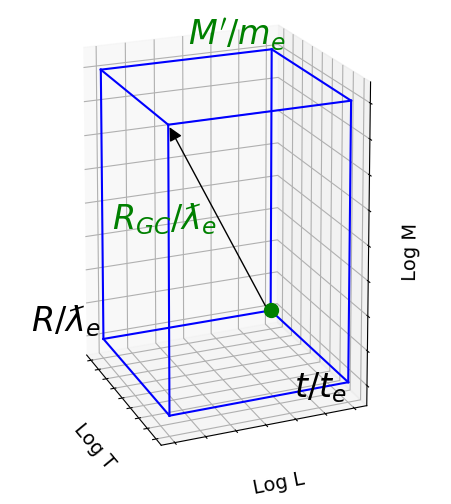
\includegraphics[width=5cm,height=6cm]{./figures/triaxis.png} 
\caption[Representation Geo-dimensionelle du couple Univers-Grandcosmos]{Representation Geo-dimensionelle du couple Univers-Grandcosmos. Dans un super espace 3D, les logarithmes naturels de temps, de longueurs et de masses sont considérés comme vecteurs. Le rapport logarithmique du rayon du grand cosmos avec la longueur d'onde de l'électron Compton fait apparaitre un vecteur normé projetant longueur et temps avec une proportion commune; le rayon de Hubble par la longueur d'onde de l'électron Compton et pour le rapport de masse; on considere $M^{\prime}$ par la masse de l'électron. $M^{\prime}$ étant la masse critique dans le Grandcosmos réduit a un hologramme spherique, ceci démontre la confirmation géometrique du principe holographique étendu (2D-1D)appliqué a l'univers d'entropie de Bekenstein-Hawking. L'existence d'un grand cosmos ne peut plus \^etre niée depuis que la relation entre $e$, $a$ et les logarithmes impliqués atteignent une précision de $10^{-7}$.}
  %\label{fig:figure_label}
\label{fig:1:figure1}
\end{figure}

\begin{figure}
\centering
% \fbox{\rule[-.5cm]{4cm}{4cm} \rule[-.5cm]{4cm}{0cm}}
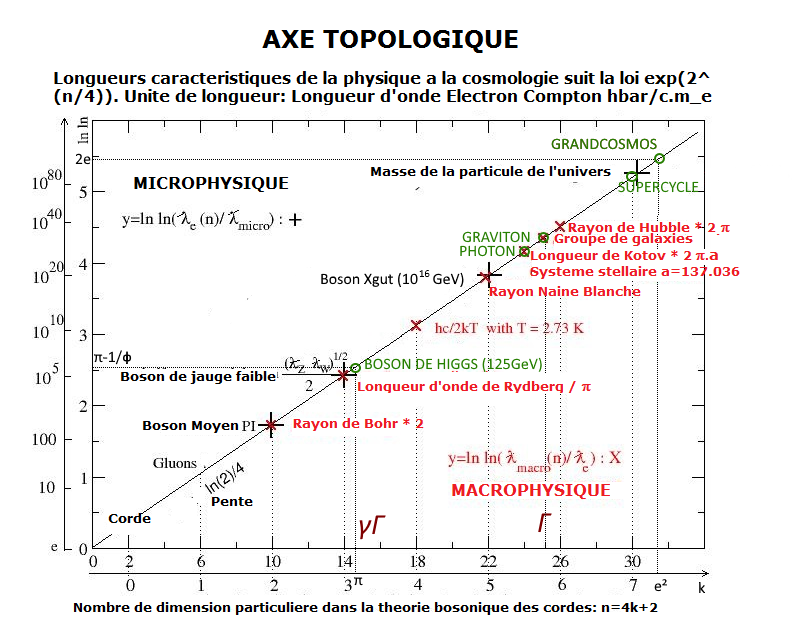
\includegraphics[width=15cm,height=16cm]{./figures/figure.png}
\caption[Axe Topologique]{L'axe topologique. Le double logarithme naturel (y = lnln(Y)) de quantités physique sans dimensions (Y) corresponds à la corde dimensionelle de series n = 4k + 2, de k = 0 a k = 7, montrant la périodicité de Bott qui est à l'origine du nom Axe Topologique.}
\label{fig:2:figure2}
\end{figure}

\begin{figure}[h]
\centering
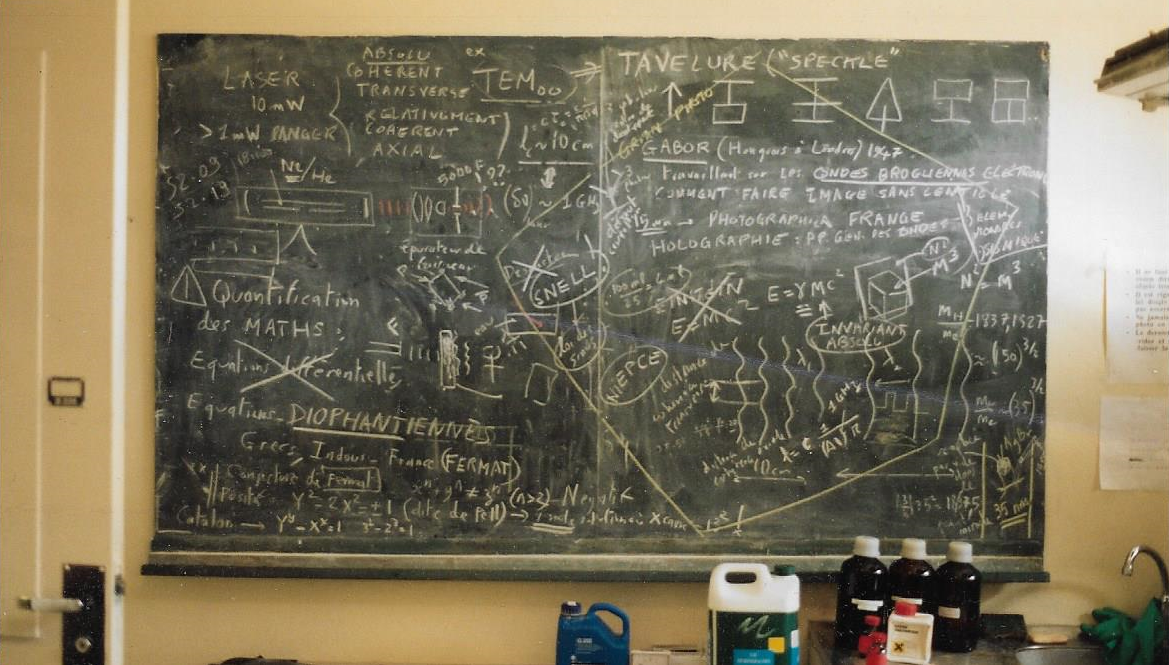
\includegraphics[width=14.5cm,height=10.5cm]{./figures/fs-tab.png}
\caption [Cours d'holographie à l'Institut d'Optique d'Orsay]{\textit{Cours d'holographie de Francis M. Sanchez à l'Institut d'Optique d'Orsay fin des années 1980}, remarquer les quelques formules ainsi que les références aux équations diophantiennes.} 
\label{fig:3:figure3}
\end{figure}

%% \begin{figure}[h]
\begin{figure}
\centering
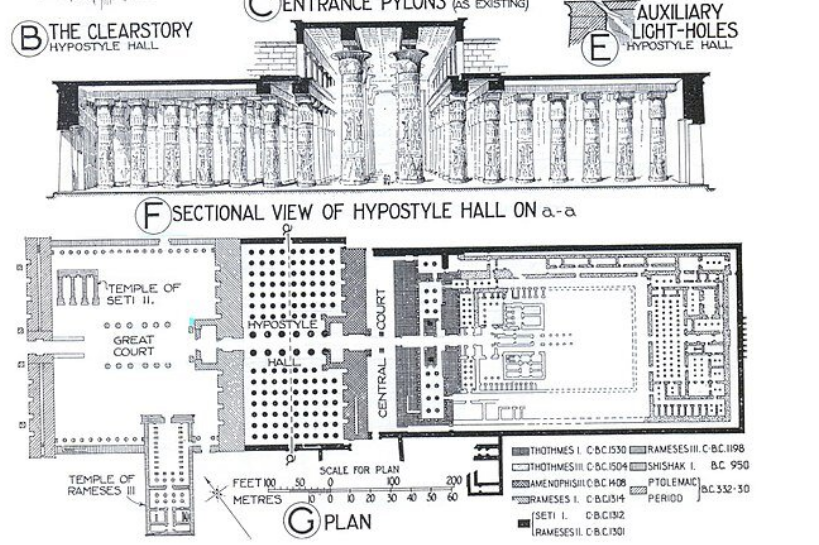
\includegraphics[width=14.5cm,height=8.6cm]{./figures/karnak.png}
\caption [Plan du Temple de Karnak]{\textit{Vue de la salle Hypostyle du Temple de Karnak en Haute Egypte} - Plan et coupe.} 
\label{fig:4:figure4}
\end{figure}

\begin{figure}
\centering
%%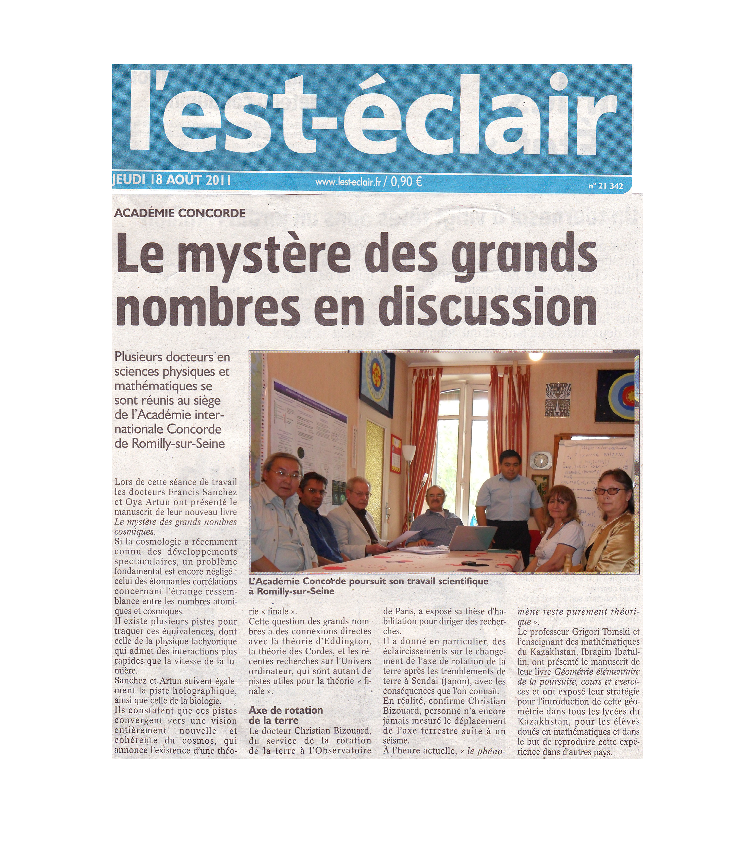
\includegraphics[width=13.5cm,height=11.0cm]{./figures/lesteclair.png}
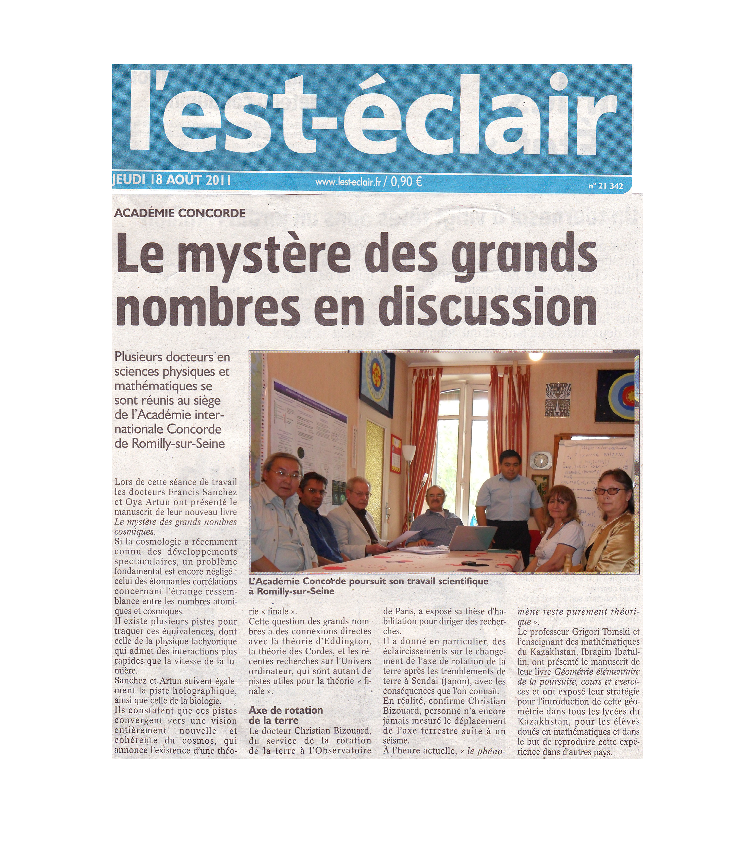
\includegraphics{./figures/lesteclair.png}
\caption [L'est-Eclair: Le mystere des grands nombres]{\textit{Le mystere des grands nombres} - Article du quotidien regional l'Est-Eclair du 18 Ao\^ut 2011.} 
\label{fig:5:figure5}
\end{figure}


%% \begin{figure}[h]
\begin{figure}
\centering
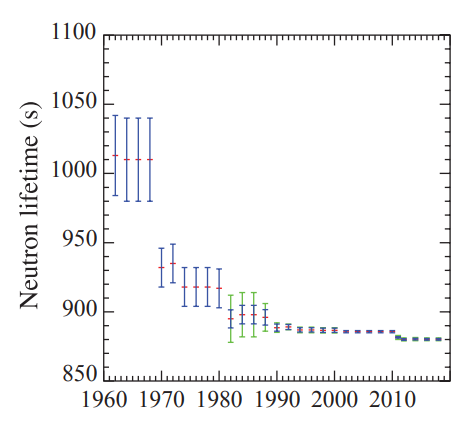
\includegraphics[width=13.5cm,height=8.6cm]{./figures/neutron-lifetime-pdg.png}
\caption[Mesures de la duree de vie du neutron depuis 1962]{\textit{Duree de vie du Neutron d'apres Particle Data Group 2019} - Tracé historique.} 
\label{fig:6:figure6}
\end{figure}

\begin{figure}
\centering
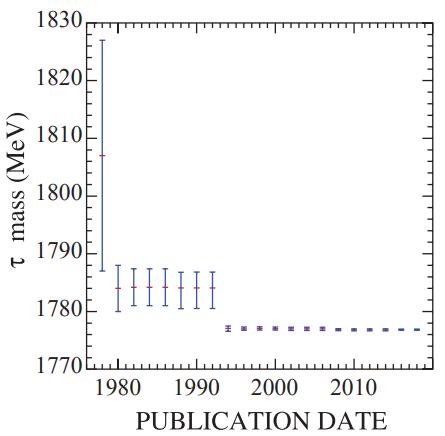
\includegraphics[width=13.5cm,height=8.6cm]{./figures/tau-mass-pdg.png}
\caption [Mesures de la masse du Tau depuis 1978]{\textit{Mesure de la masse du Tau d'apres Particle Data Group 2019} - Tracé historique.} 
\label{fig:7:figure7}
\end{figure}

\begin{figure}
\centering
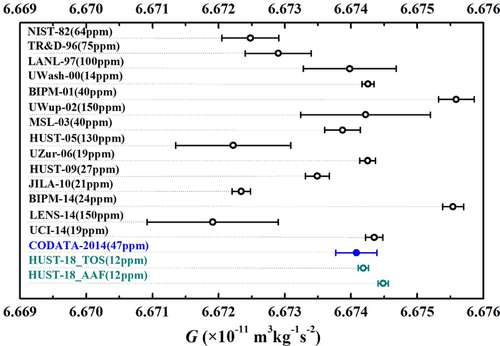
\includegraphics[width=14.5cm,height=8.6cm]{./figures/ProgressinPreciseMeasurementsoftheGravitationalConstant.png}
\caption[Mesures de la constante de gravitation G depuis 1982]{\textit{Mesures de la constante de gravitation G depuis 1982 d'apres Progress in Precise Measurements of the Gravitational Constant \cite{Wu}} - Tracé historique.} 
\label{fig:8:figure8}
\end{figure}

\begin{figure}
\centering
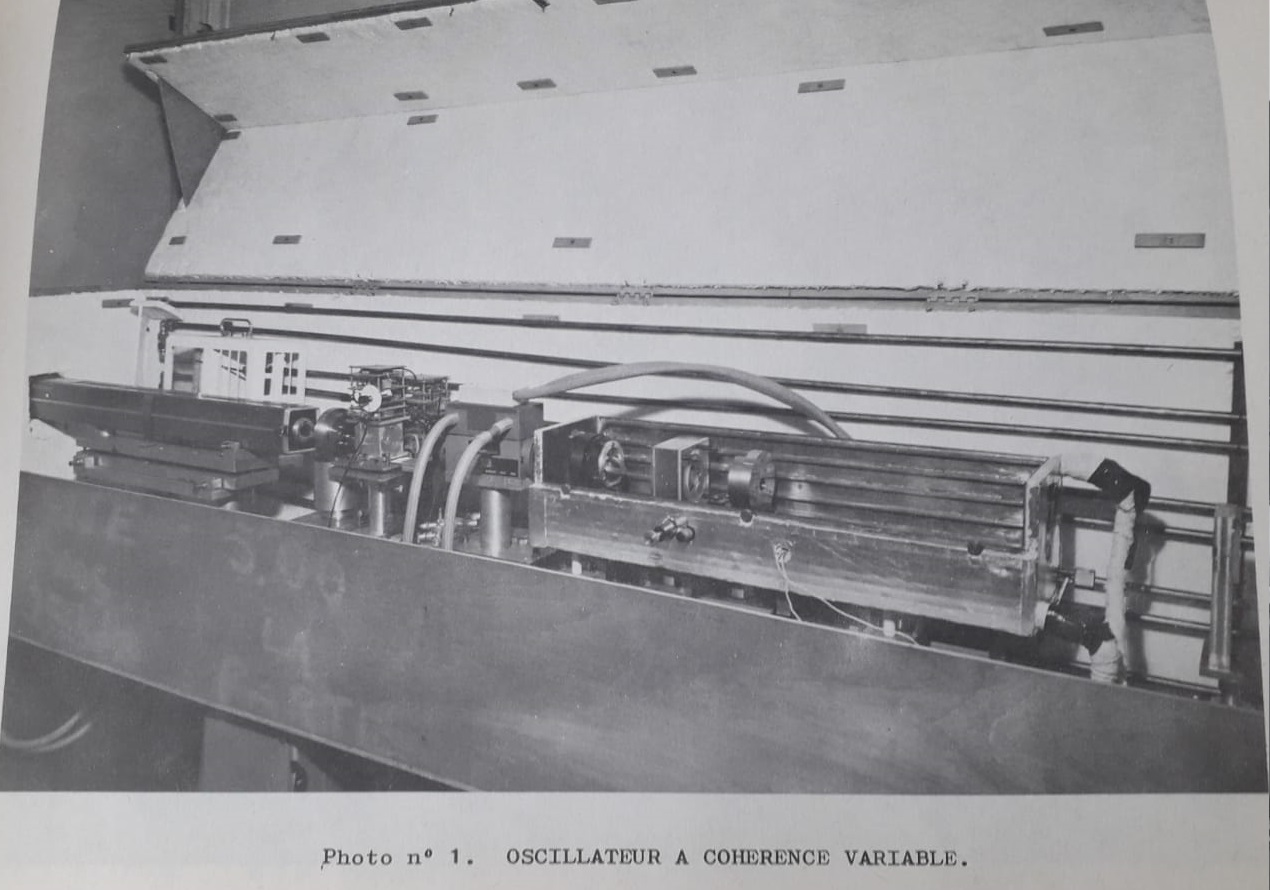
\includegraphics[width=14.5cm,height=8.6cm]{./figures/oscillateur-CEA-multiphotonGroup.jpg}
\caption[Vue de l'oscillateur du LASER $Nd^{3p+}$]{\textit{Oscillateur du LASER $Nd^{3p+}$ } - Photo realise au CEA en 1973.} 
\label{fig:9:figure9}
\end{figure}

\begin{figure}
\centering
%%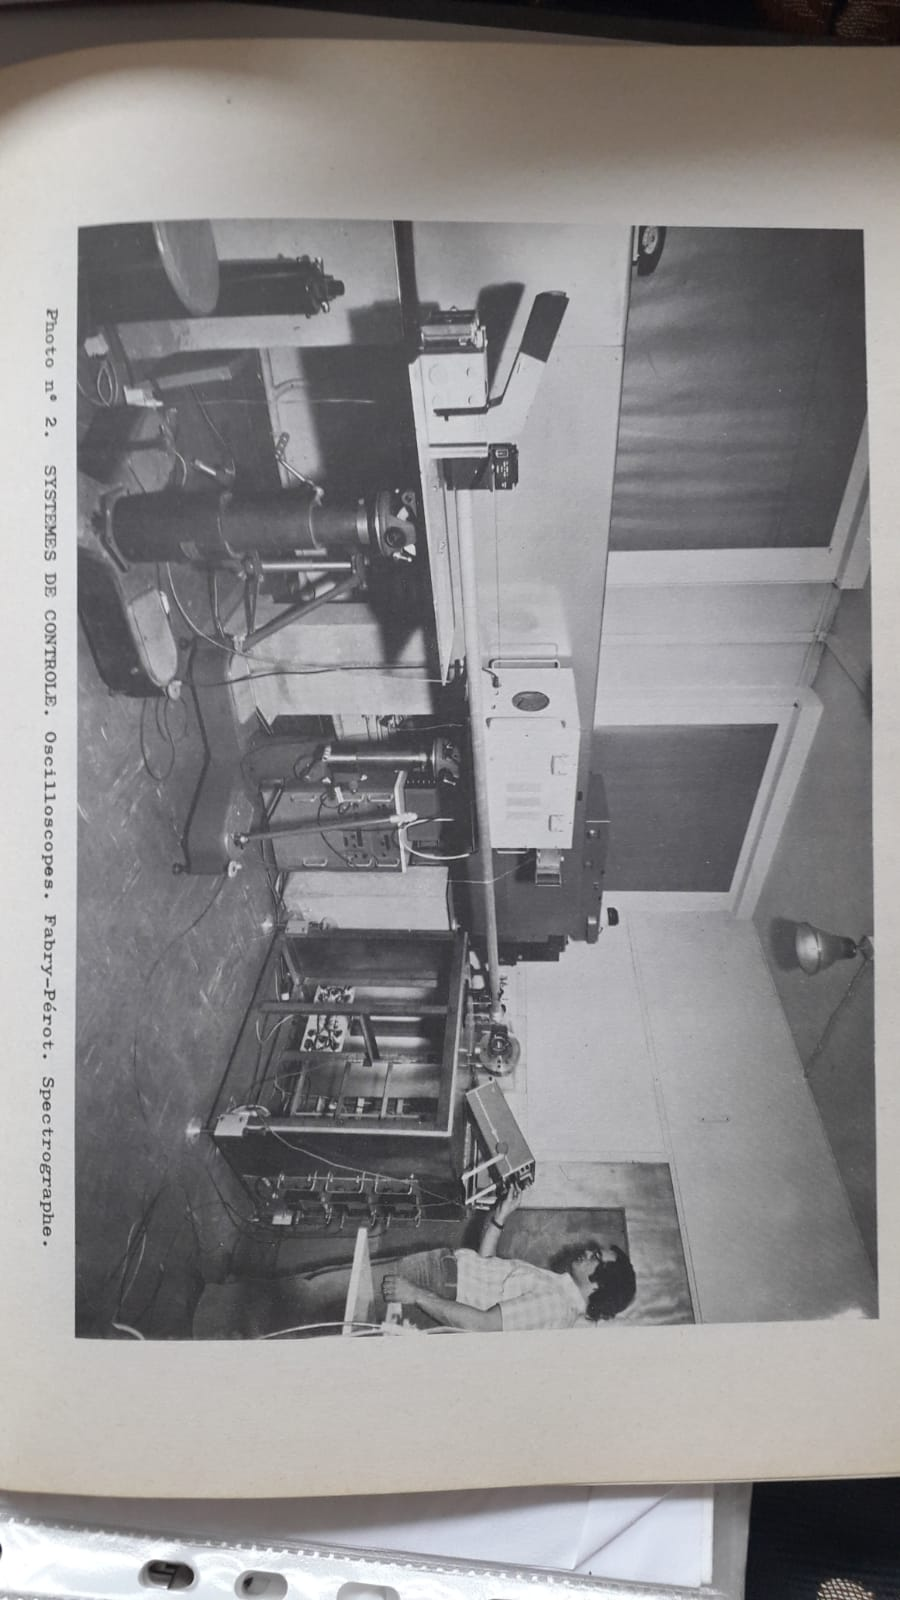
\includegraphics[width=14.5cm,height=8.6cm]{./figures/ControlSystemOscilloFabryPerot-CEA-multiphotonGroup.jpg}
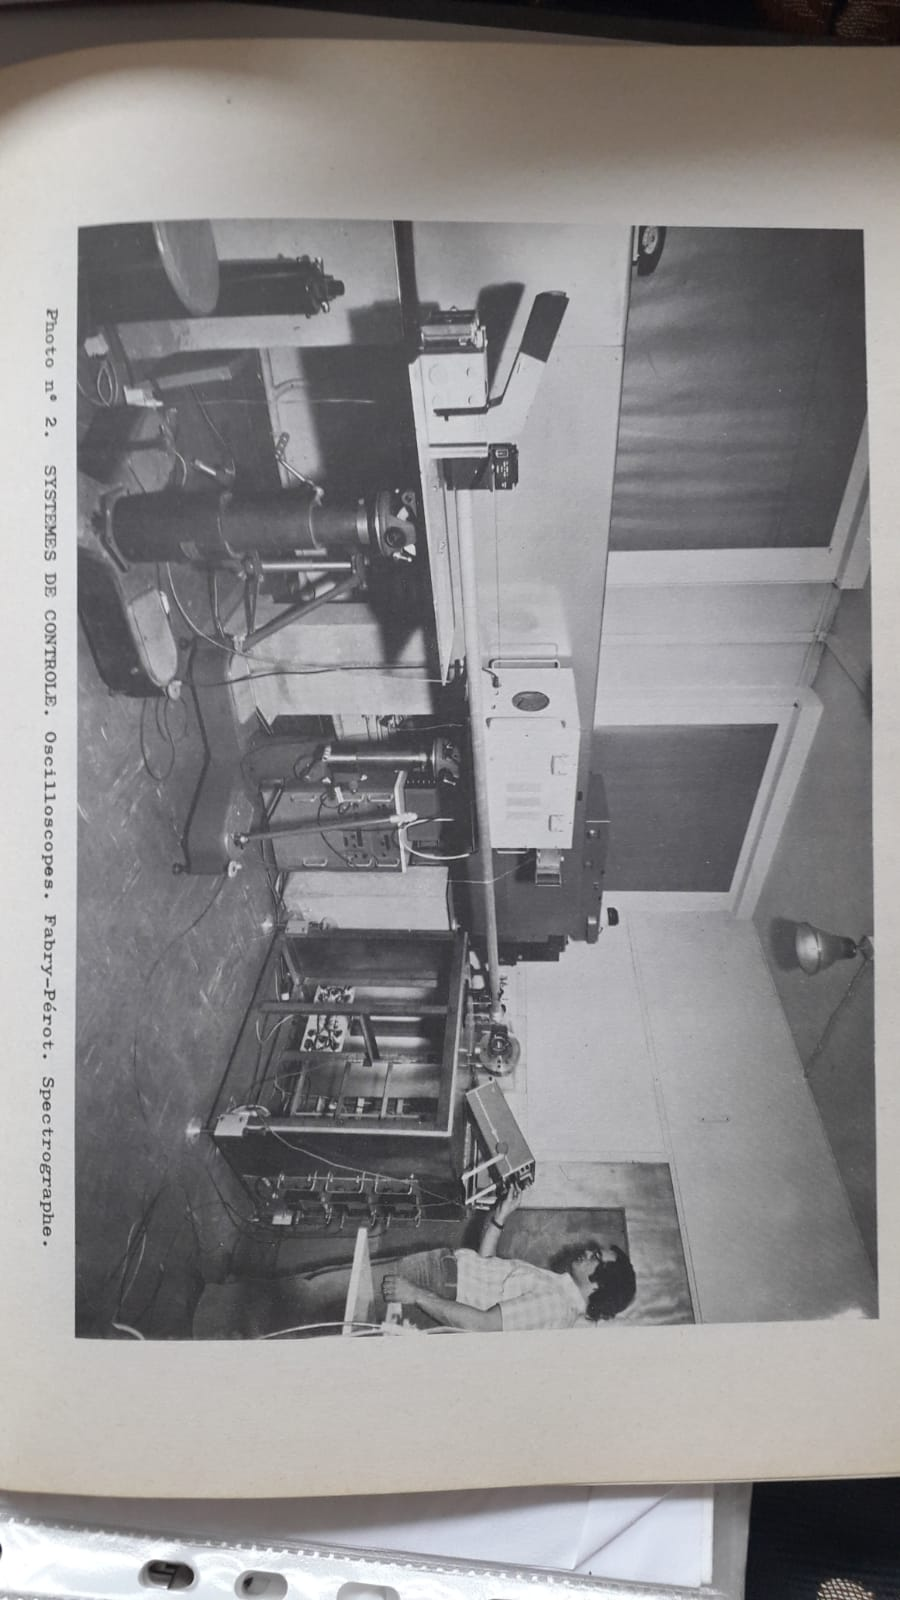
\includegraphics[width=14.5cm,height=8.6cm]{./figures/ControlSystemOscilloFabryPerot-CEA-multiphotonGroup.jpg}
\caption[Vue du systeme de controle du LASER $Nd^{3p+}$]{\textit{Systeme de controle du LASER $Nd^{3p+}$ muni d'oscilloscope, de spectrographe et de cavite Fabry-Perot} - Photo realisé au CEA en 1973.} 
\label{fig:10:figure10}
\end{figure}


\begin{figure}
\centering
\includegraphics[width=12.5cm,height=7.5cm]{./figures/Cambridge.jpg}
\caption[La conference de l'ANPA a Cambridge en 1995]{\textit{La conference de l'ANPA a Cambridge: 2eme rang assis de droite a gauche: Mike Manthey, Clive Kilmister, Francis Sanchez, ... debout: K. Bowden, Geoffrey Constable, Peter Marcer, ..., ..., P. Noyes} Sept 1995 }
\label{fig:11:figure11}
\end{figure}



\begin{figure}
\centering
%%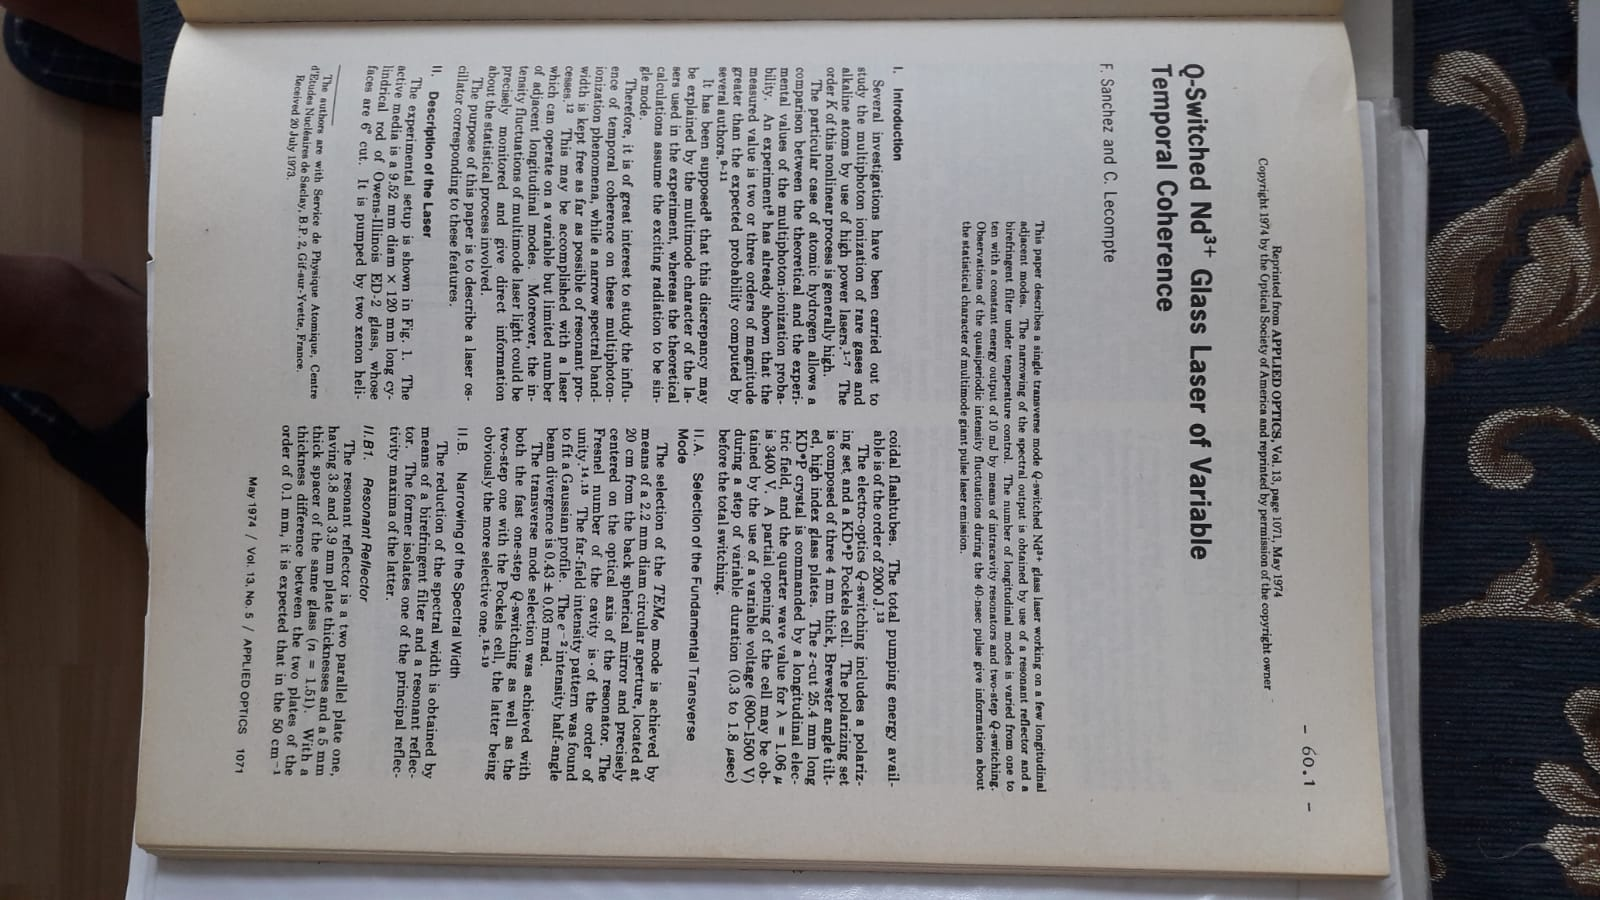
\includegraphics[width=14.5cm,height=8.6cm]{./figures/Nd3PlusGlassLASER-paper-1973.jpg}
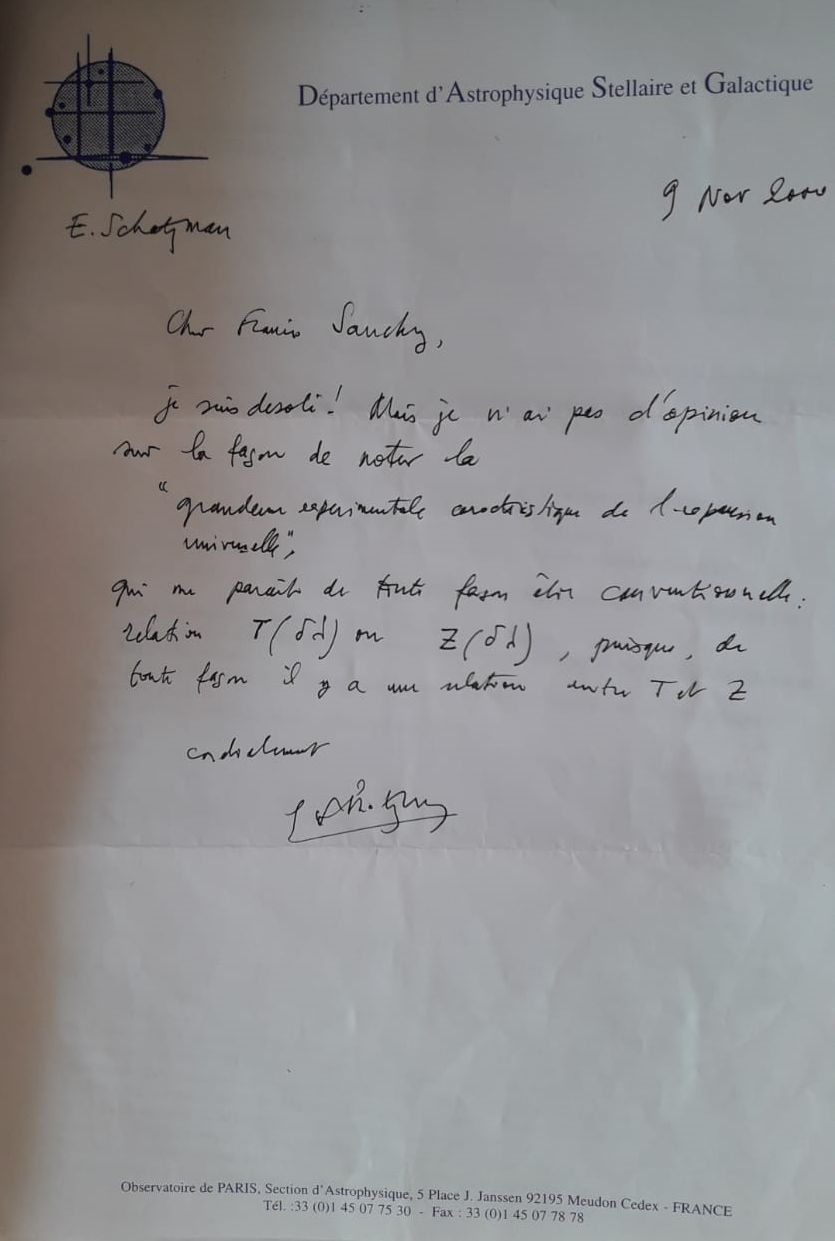
\includegraphics[width=8.5cm,height=14.5cm]{./figures/schatzmann.png}
\caption[Courrier d'evaluation de Schatzman]{\textit{Courrier de Schatzman du Département d'Astrophysique Stellaire et Galactique évaluant le rapport sur la cosmologie de Francis M. Sanchez} - 9 Nov 2000.} 
\label{fig:12:figure12}
\end{figure}


\begin{figure}
\centering
%%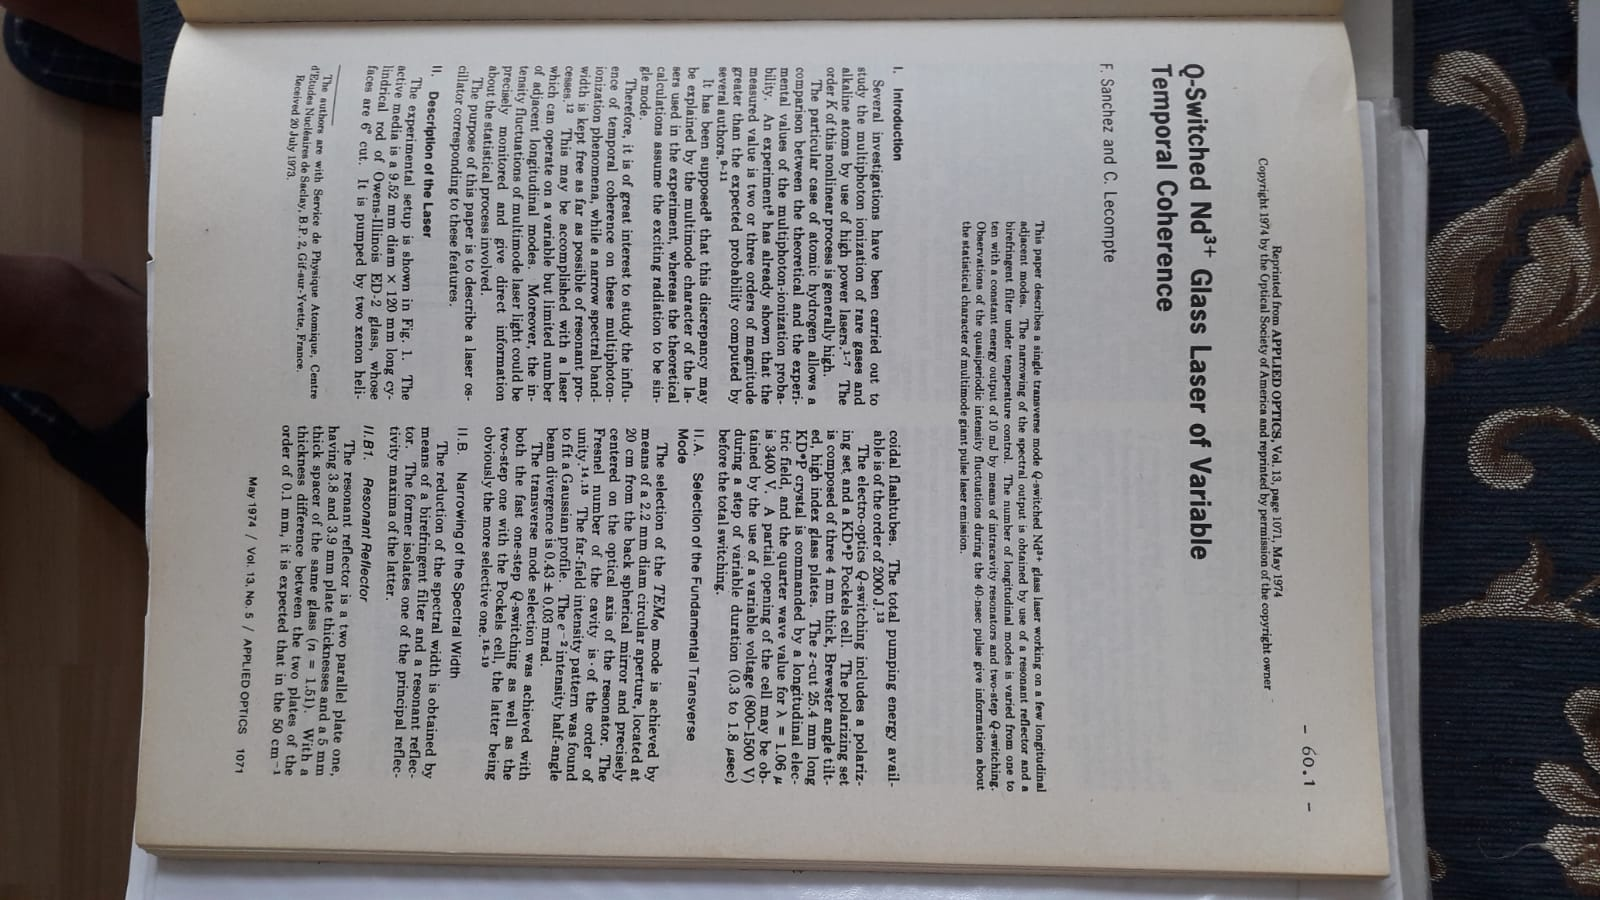
\includegraphics[width=14.5cm,height=8.6cm]{./figures/Nd3PlusGlassLASER-paper-1973.jpg}
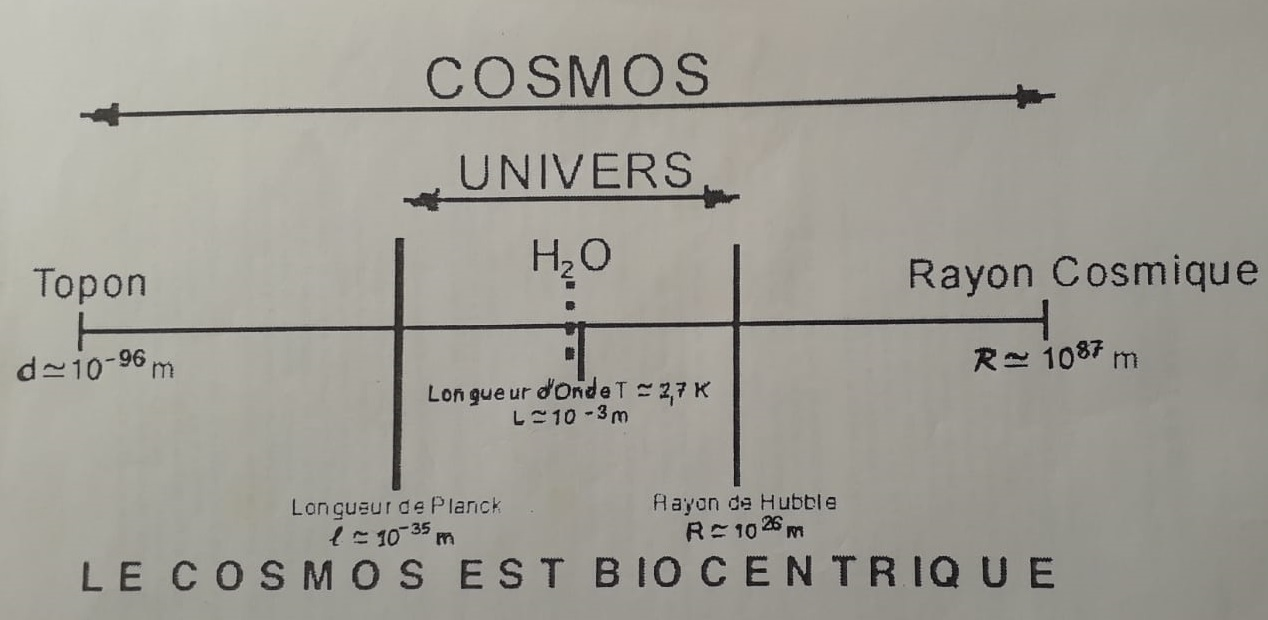
\includegraphics[width=14.5cm,height=8.5cm]{./figures/h2o-biocentrique.jpg}
\caption[Schema du Cosmos Biocentrique $H_2O$ ]{\textit{Schema du cosmos biocentrique autour de $H_2O$} - 9 Nov 2000.} 
\label{fig:13:figure13}
\end{figure}

\begin{figure}
\centering
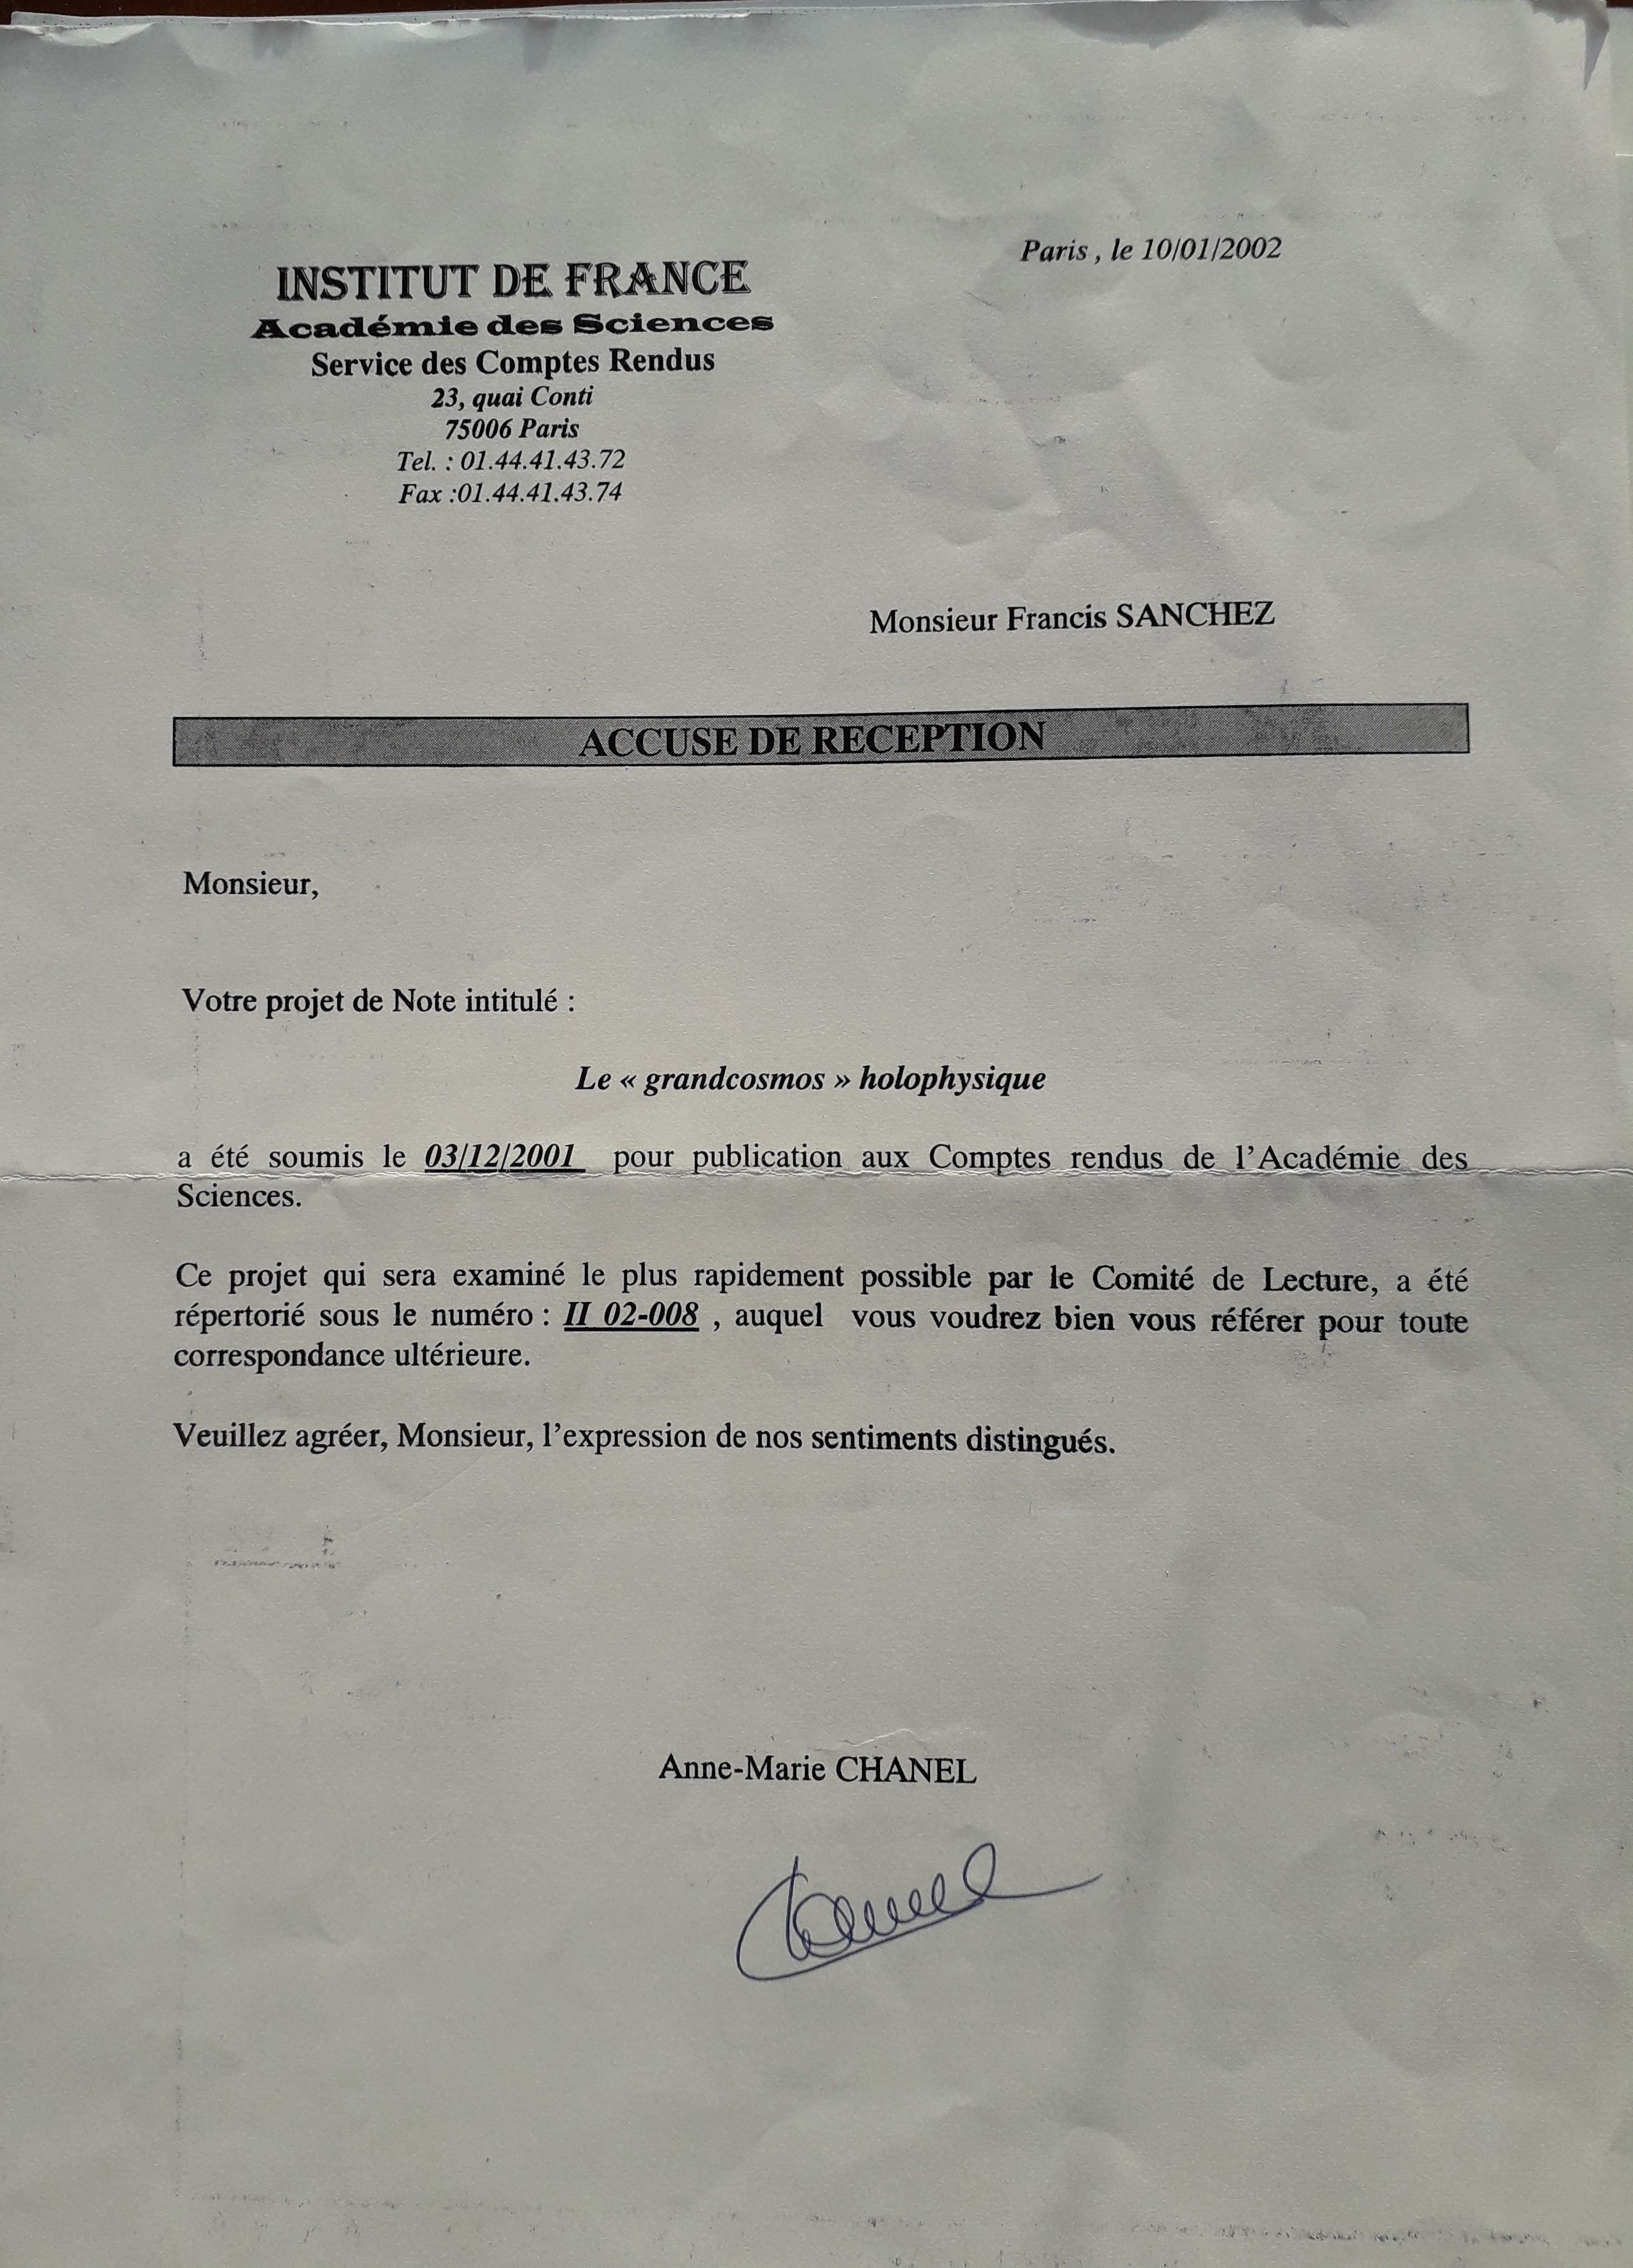
\includegraphics[width=8.5cm,height=14.5cm]{./figures/AcadSciences2001.jpg}
\caption[Accuse reception du depot du compte-rendu aupres de l'Academie des Sciences]{\textit{Accuse reception du compte-rendu intitulé ``Le Grandcosmos Holophysique'' déposé aupres de l'Académie des Sciences par l'intermédiaire de l'institut de France} - 03 DEC 2001.} 
\label{fig:14:figure14}
\end{figure}

\begin{figure}
\centering
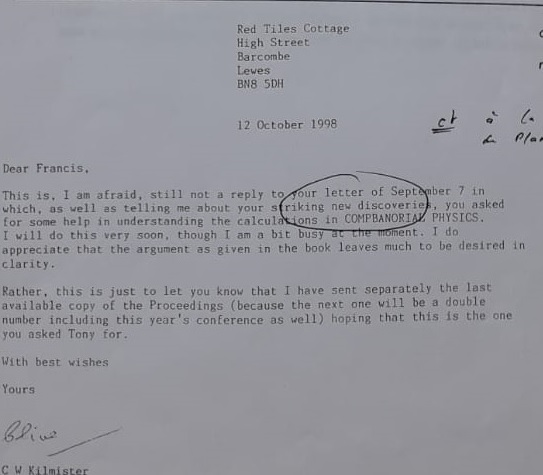
\includegraphics[width=8.5cm,height=14.5cm]{./figures/kilmister.jpg}
\caption[Rapport de Kilmister]{\textit{Rapport de Clive Kilmister} -  1998.} 
\label{fig:15:figure15}
\end{figure}

\begin{figure}
\centering
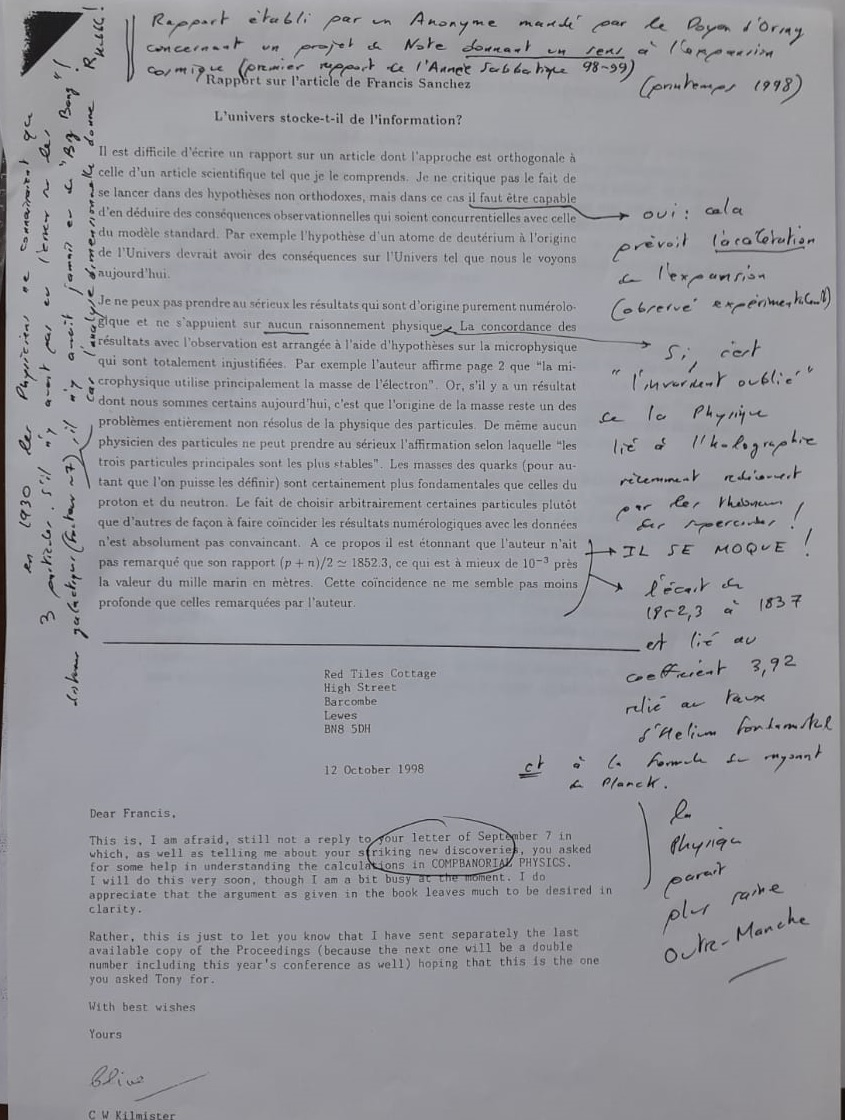
\includegraphics[width=8.5cm,height=14.5cm]{./figures/rapportAnonyme.jpg}
\caption[Rapport Anonyme demandé par le doyen de l'universite d'Orsay]{\textit{Rapport anonyme sur ``L'univers stocke-t-il de l'information ?''} -  1998.} 
\label{fig:16:figure16}
\end{figure}

\begin{figure}
\centering
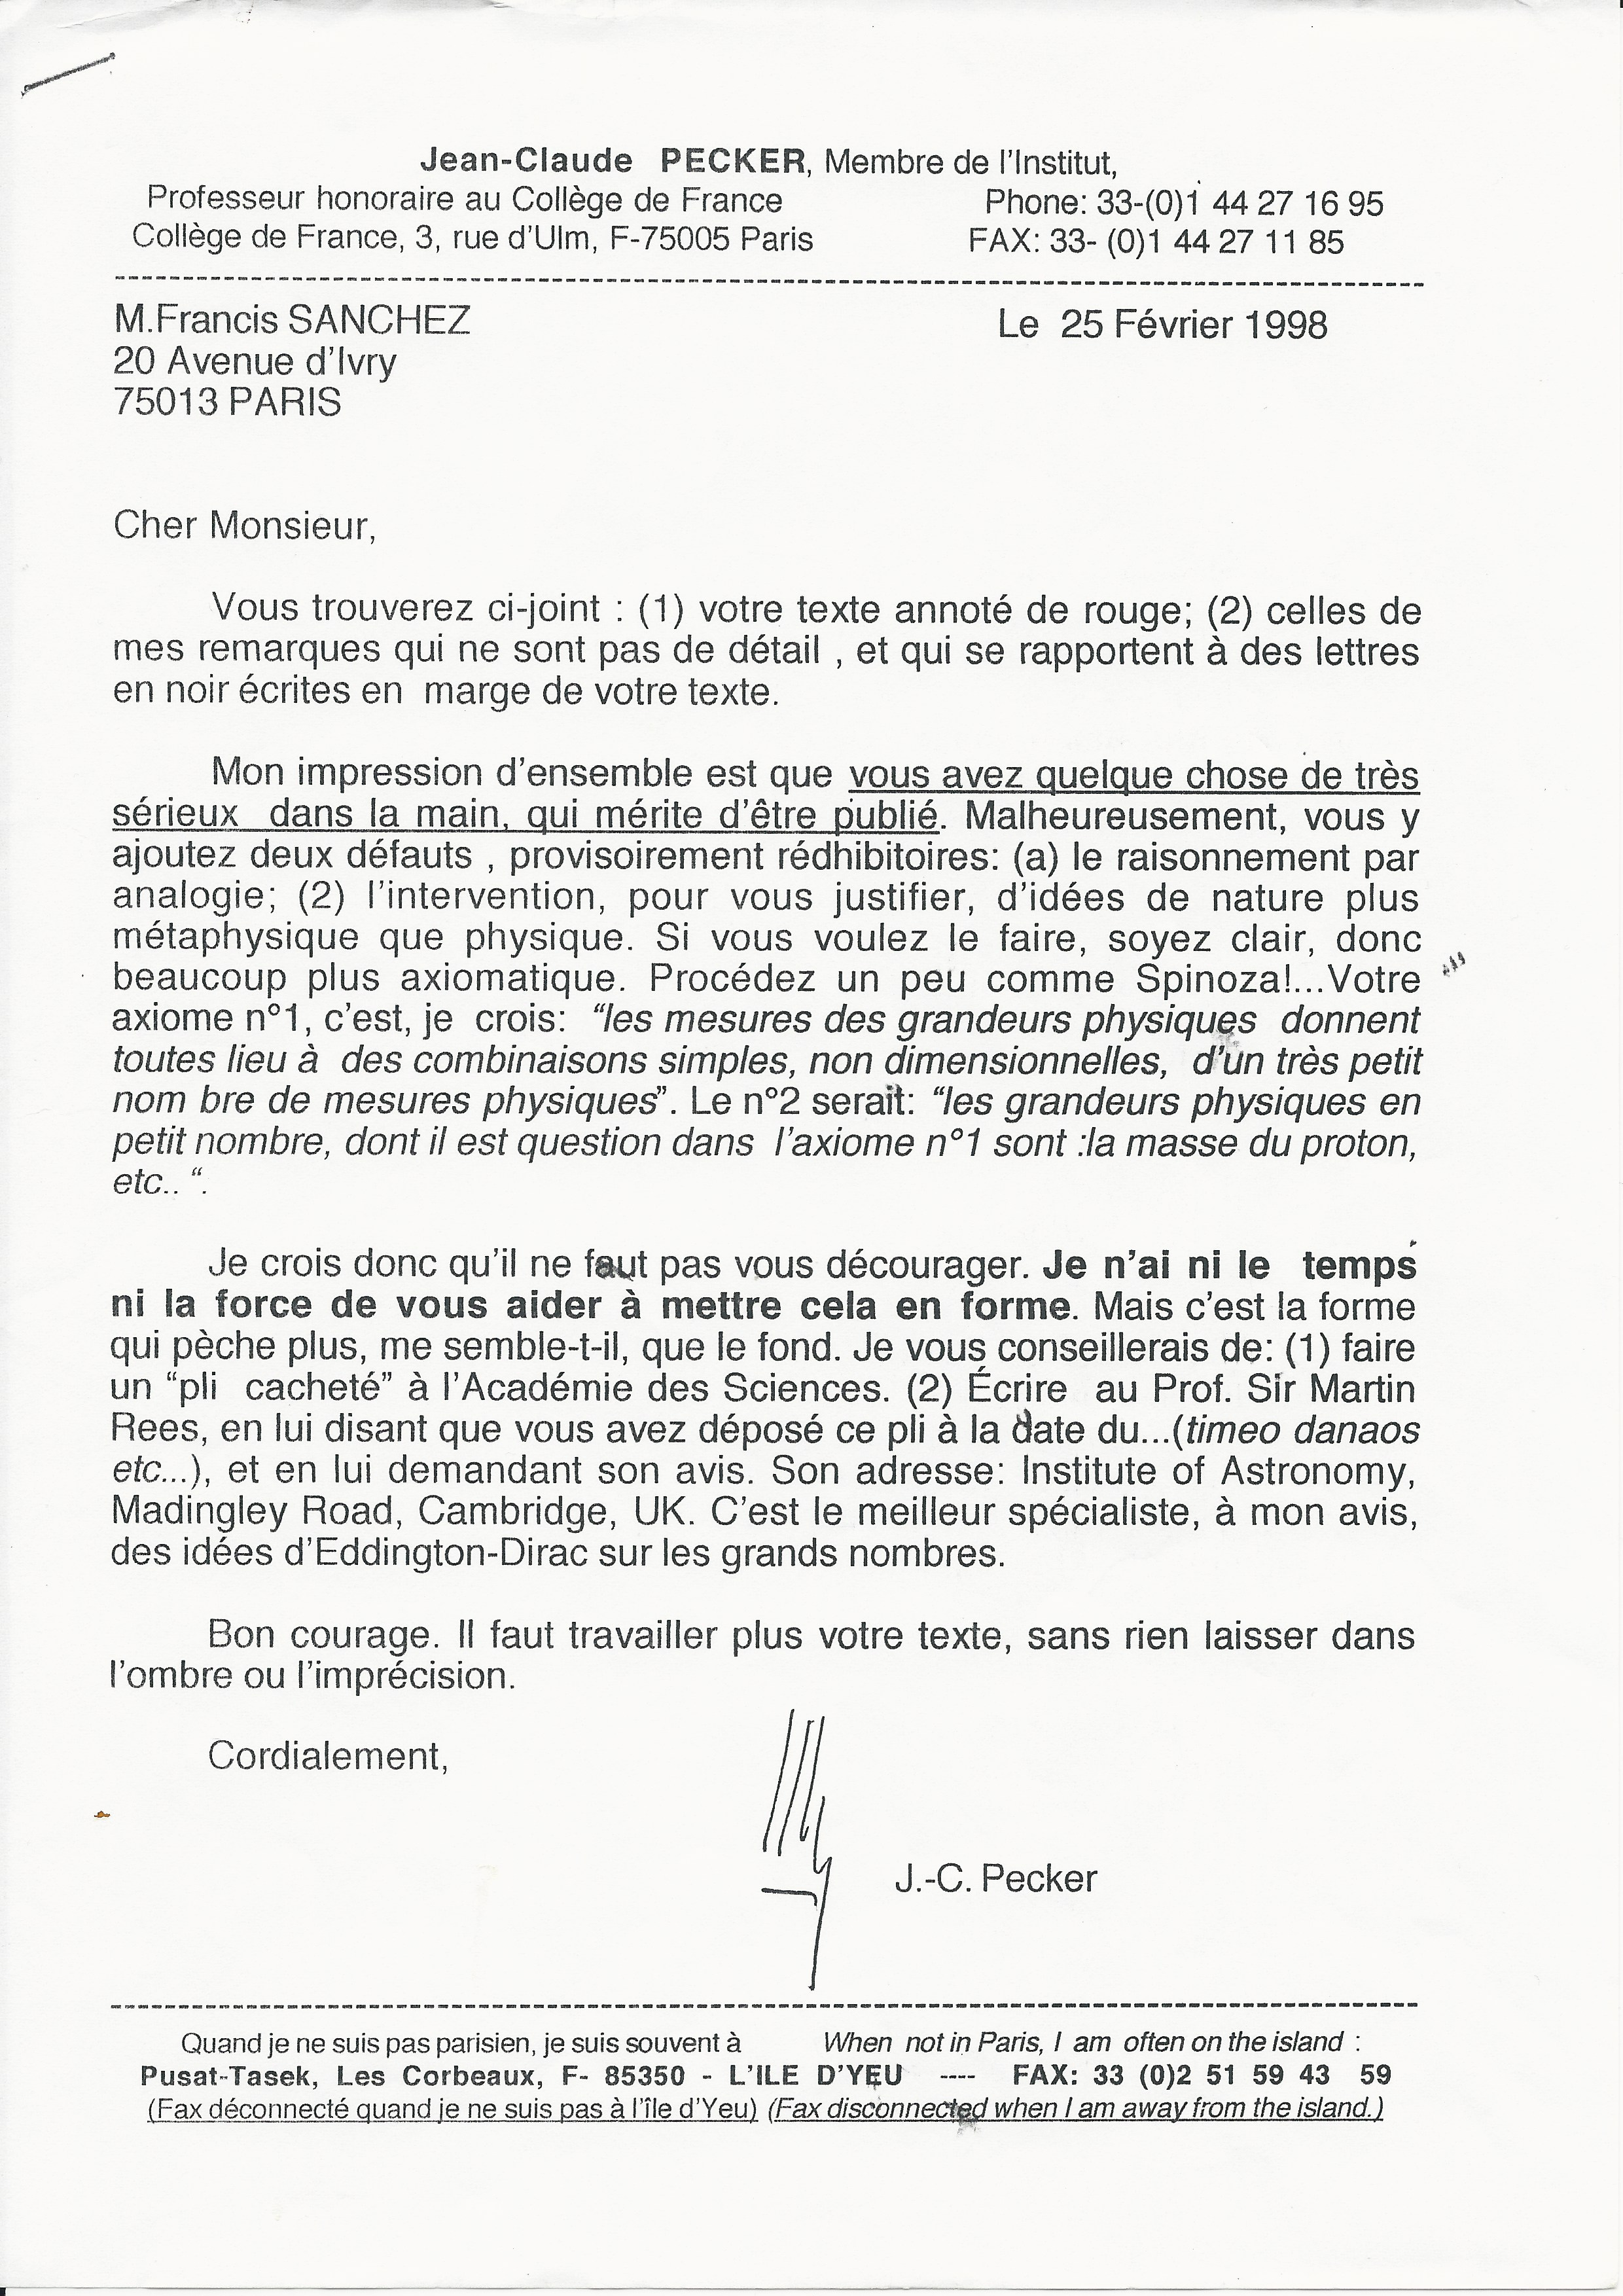
\includegraphics[width=8.5cm,height=11.5cm]{./figures/Pecker98.jpg}
\caption[Rapport de JC Pecker évaluant le travail en cosmologie de Francis M. Sanchez]{\textit{Rapport de J-C Pecker membre de l'Institut professeur honoraire au college de France} - 25 Fev 1998.} 
\label{fig:17:figure17}
\end{figure}


\begin{figure}
\centering
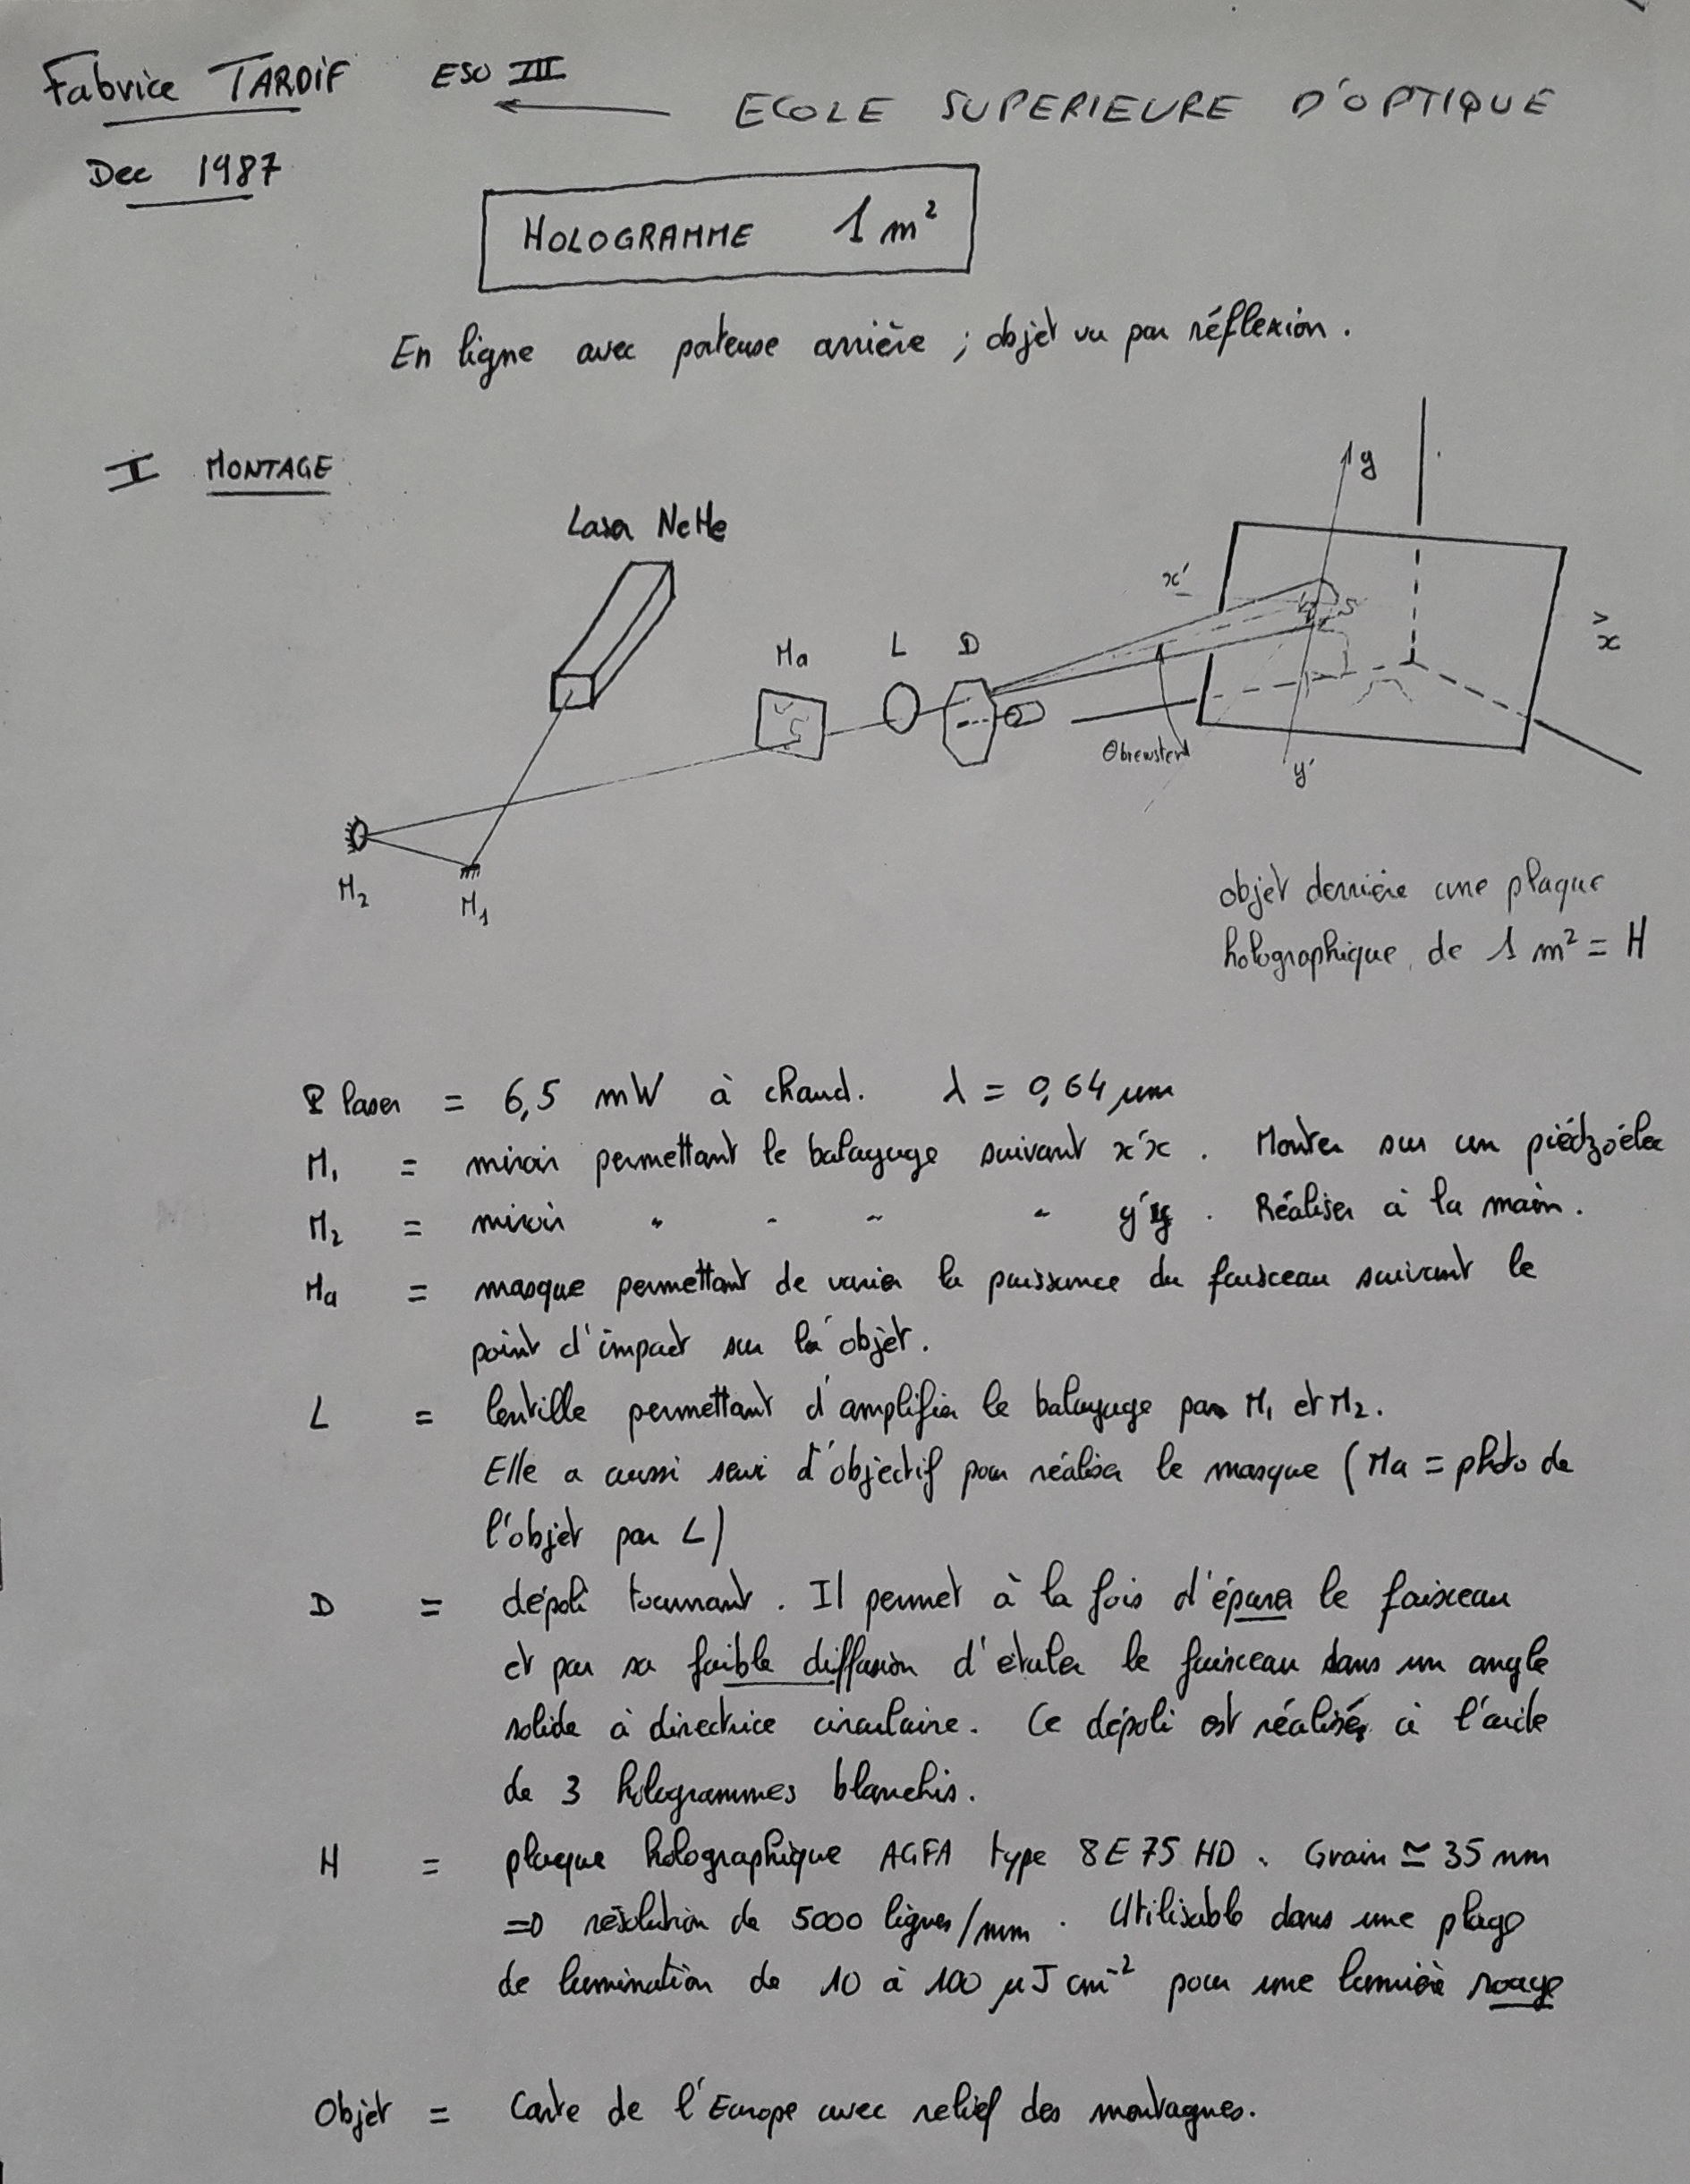
\includegraphics[width=8.5cm,height=11.5cm]{./figures/Tardif1987.png}
\caption[Rapport de Fabrice Tardif sur l'holographie à balayage]{\textit{Rapport de Fabrice Tardif sur l'holographie à balayage} décembre 1987}
\label{fig:18:figure18}
\end{figure}

\begin{figure}
\centering
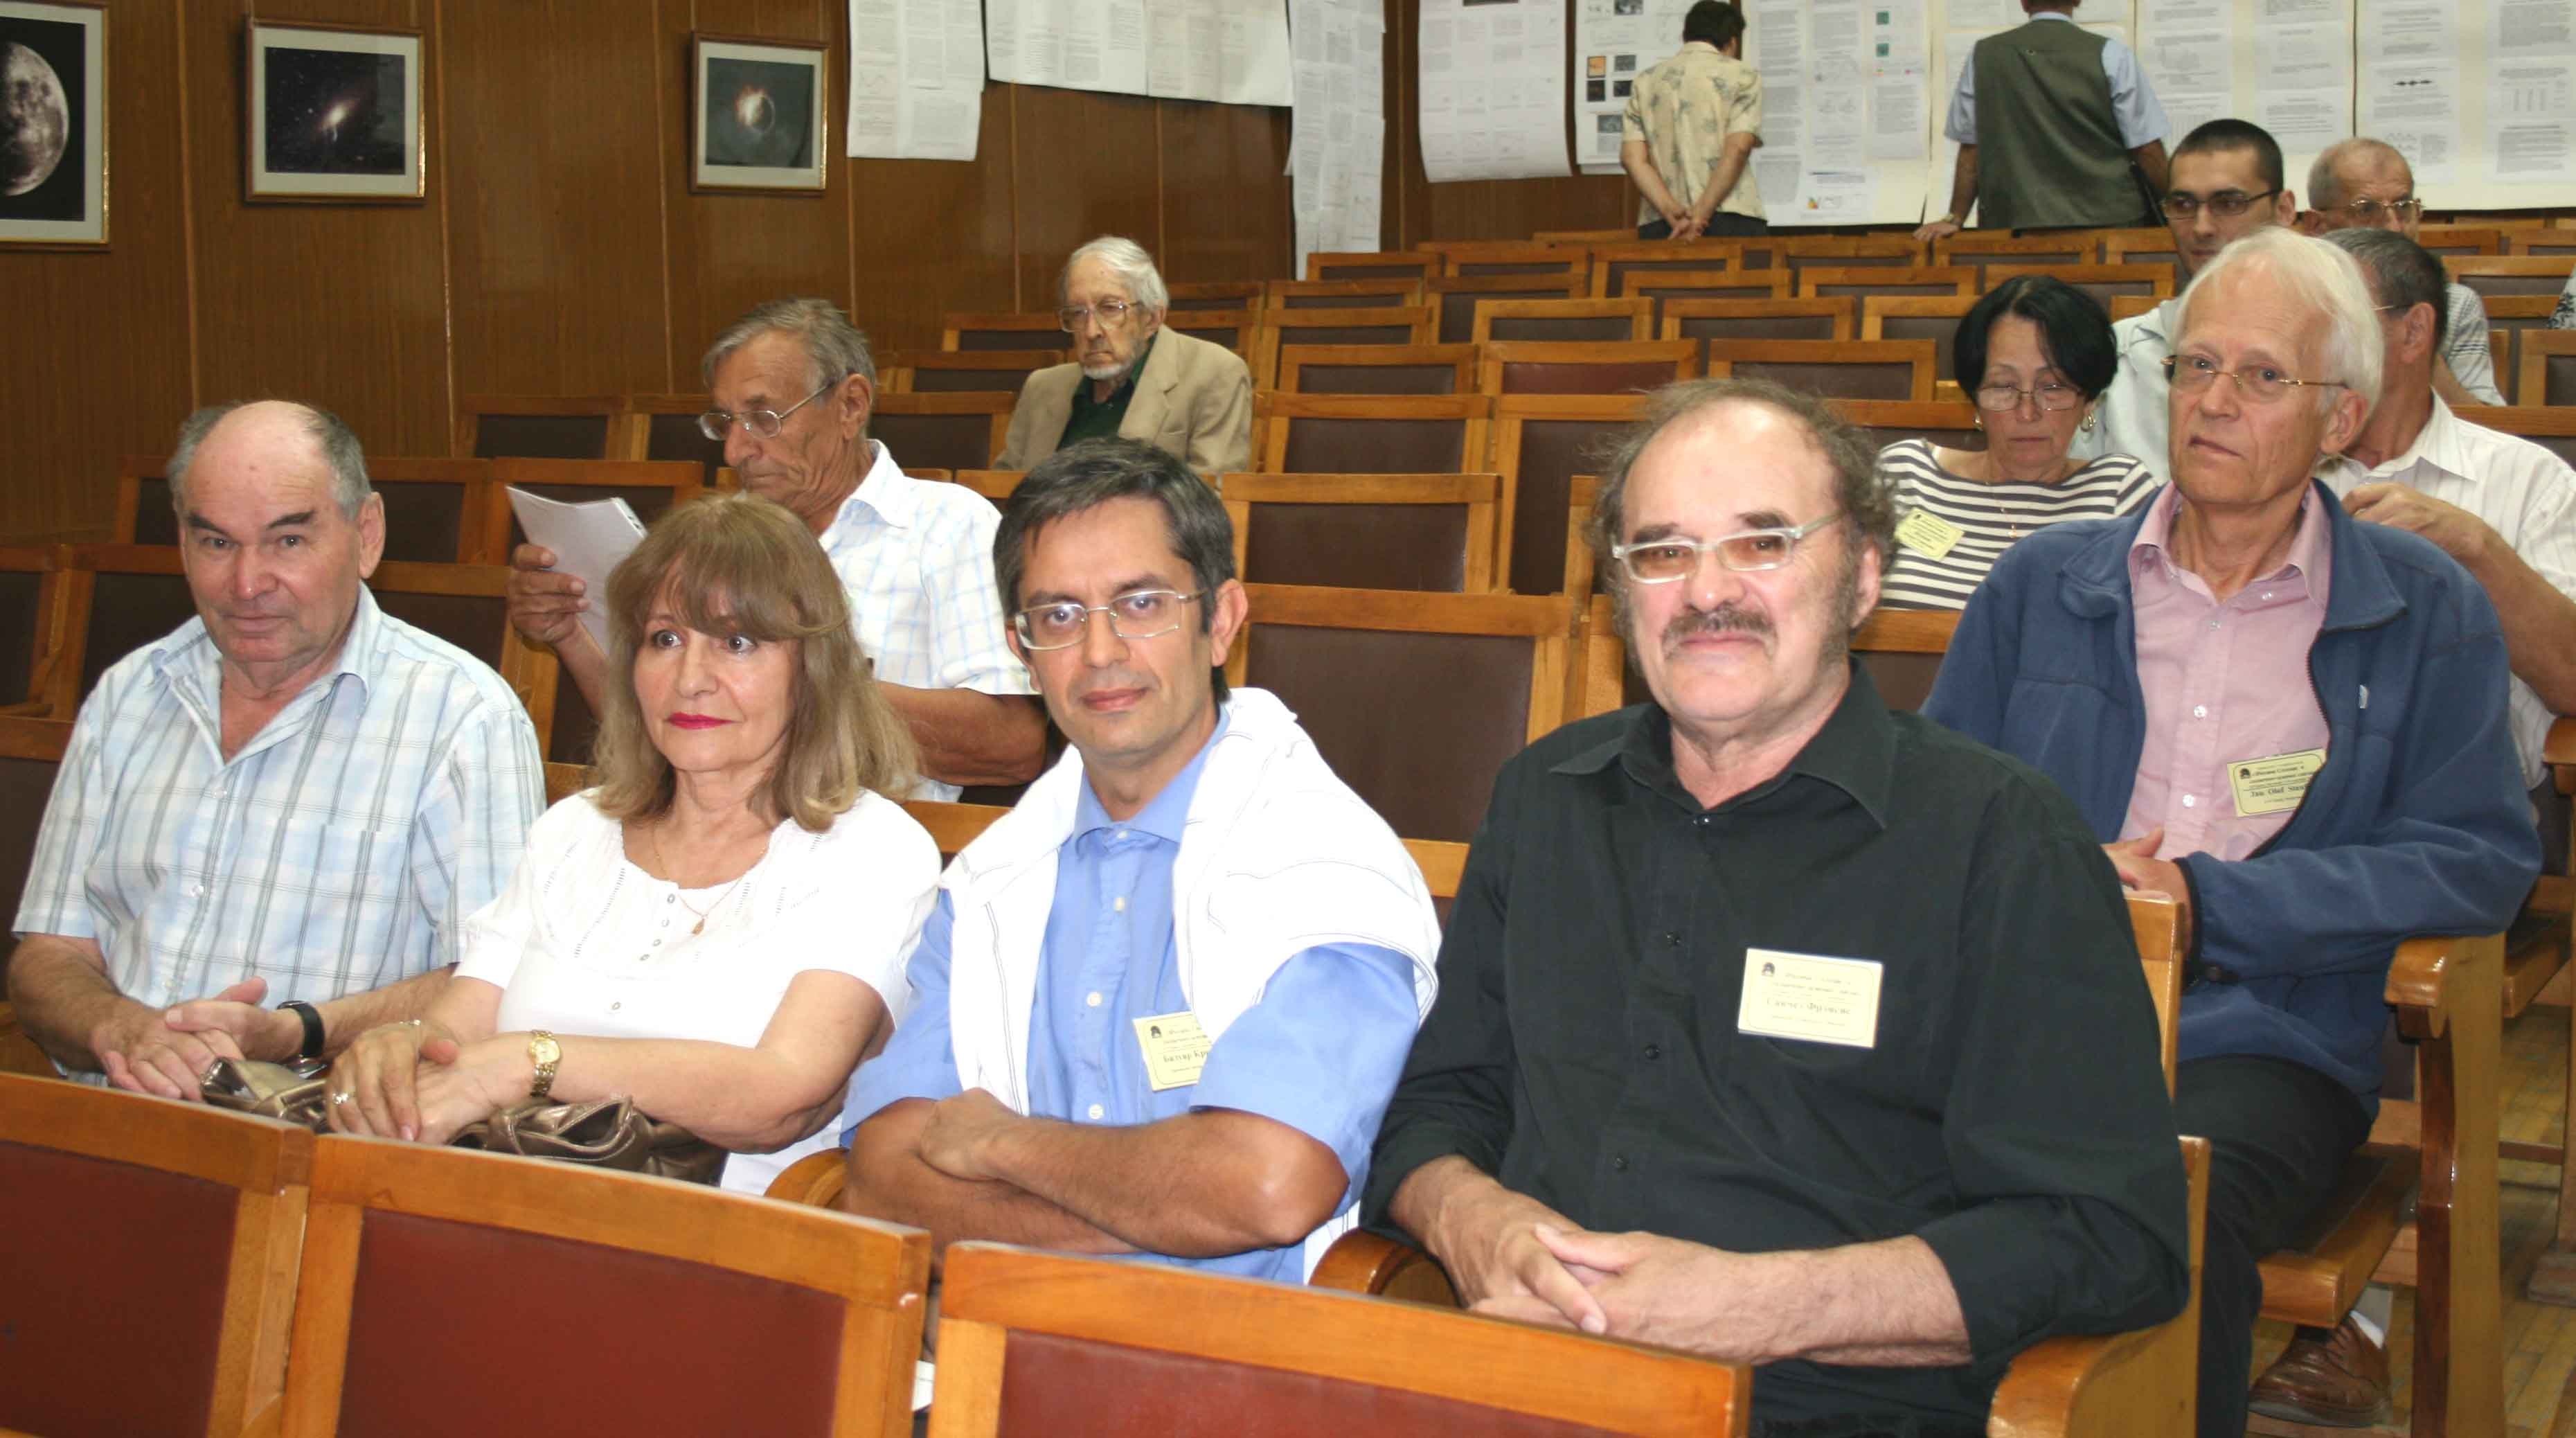
\includegraphics[width=12.5cm,height=7.5cm]{./figures/Kotov.jpg}
\caption[Réunion à l'observatoire de Crimée]{\textit{La réunion à l'observatoire de Crimée: 1er rang de droite a gauche: Francis Sanchez, Christian Bizouard, Oya Artun, Valery Kotov. 2ieme rang à droite Jan  directeur de l'Observatoire. } 2008}
\label{fig:19:figure19}
\end{figure}

\begin{figure}
\centering
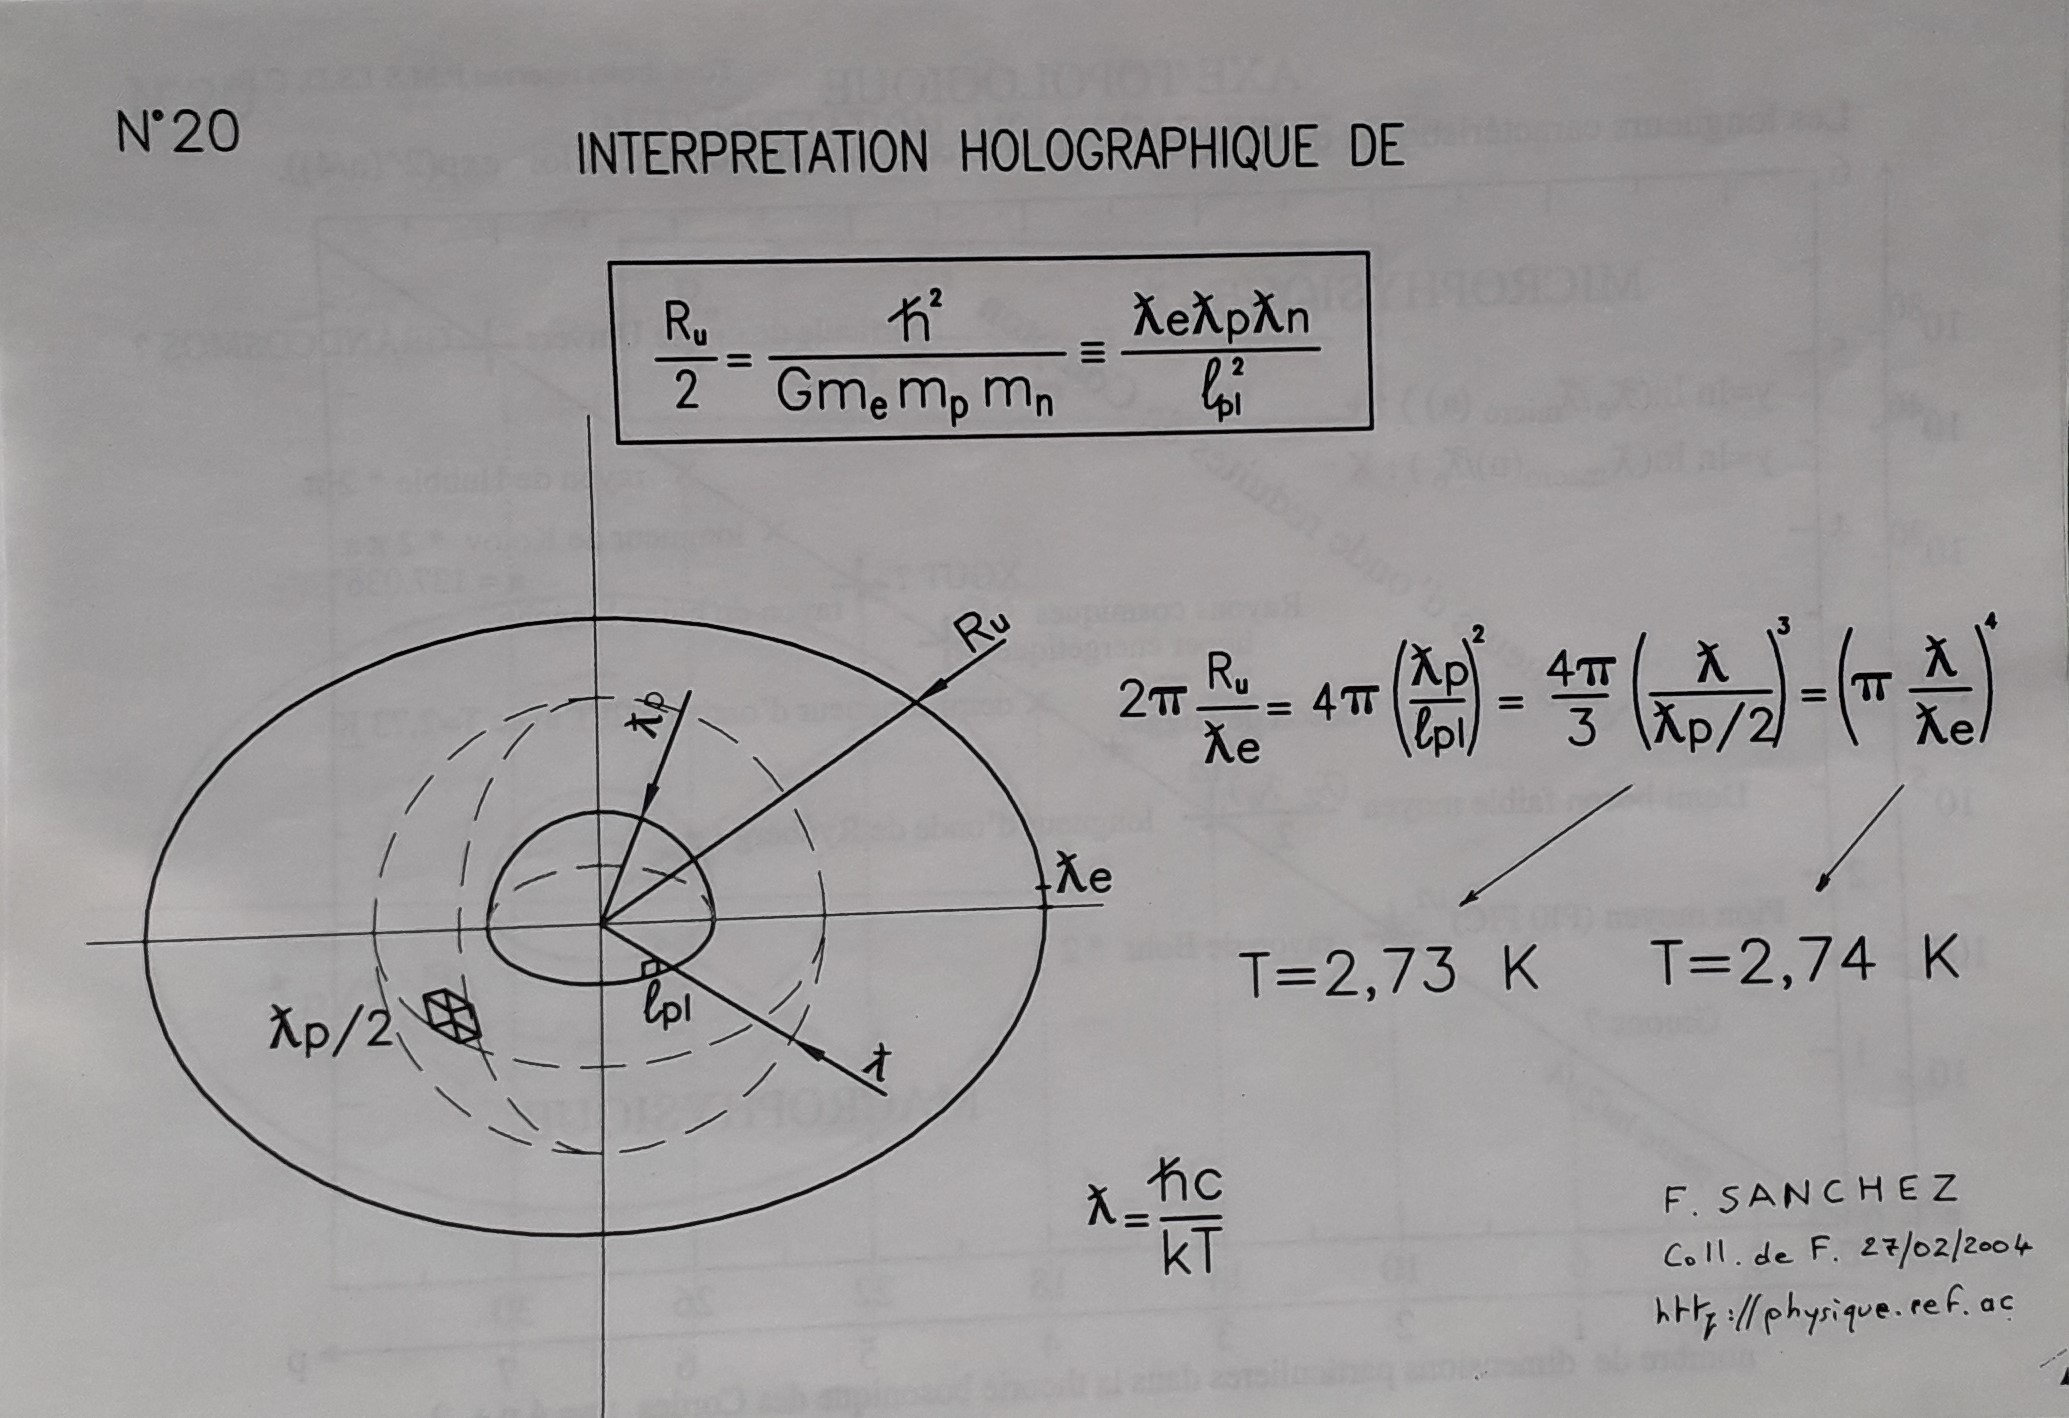
\includegraphics[width=5.5cm,height=2.6cm]{./figures/Holotemperature.jpg}
\caption[Interprétation holographique de la relation centrale. College de France]{\textit{Interprétation holographique de la relation centrale. Collège de France} Février 2004}
\label{fig:20:figure20}
\end{figure}

\begin{figure}
\centering
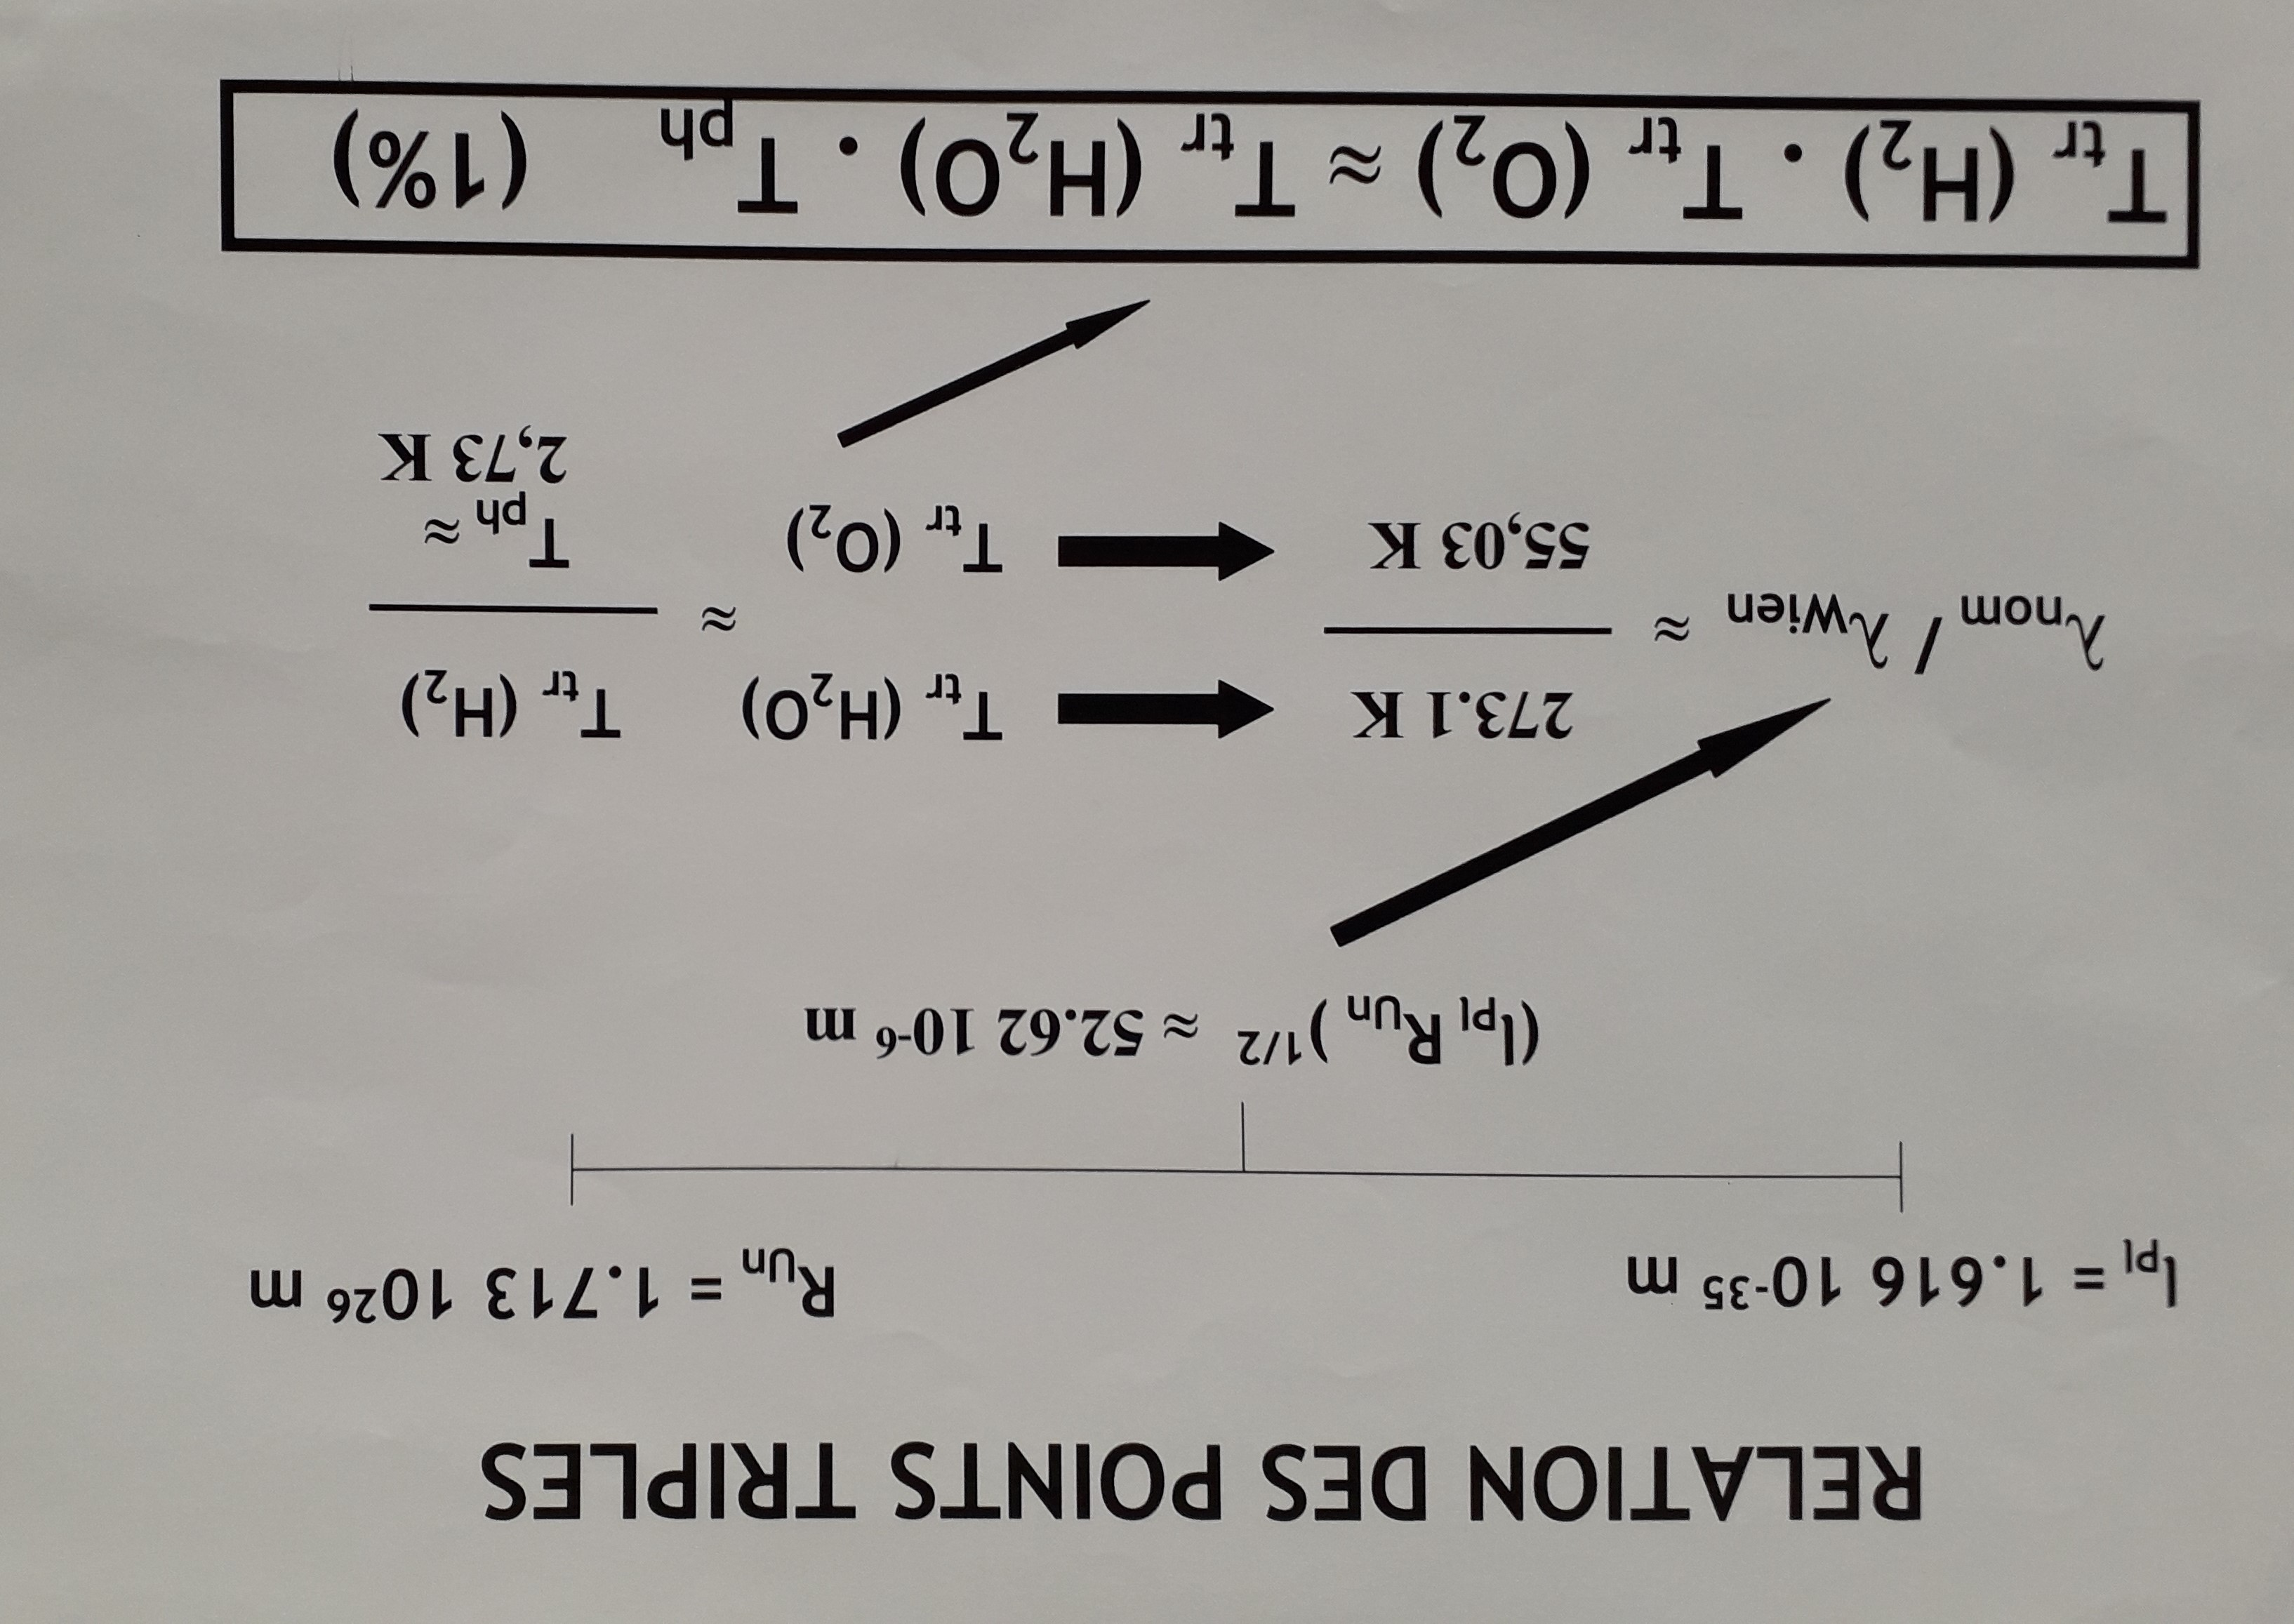
\includegraphics[width=5.5cm,height=2.5cm]{./figures/Zpointstriples.png}
\caption[Relation des Points Triples de l eau]{\textit{Relation des Points Triples de $H_2O$} - Collège de France 2004.} 
\label{fig:21:figure21}
\end{figure}

\begin{figure}
\centering
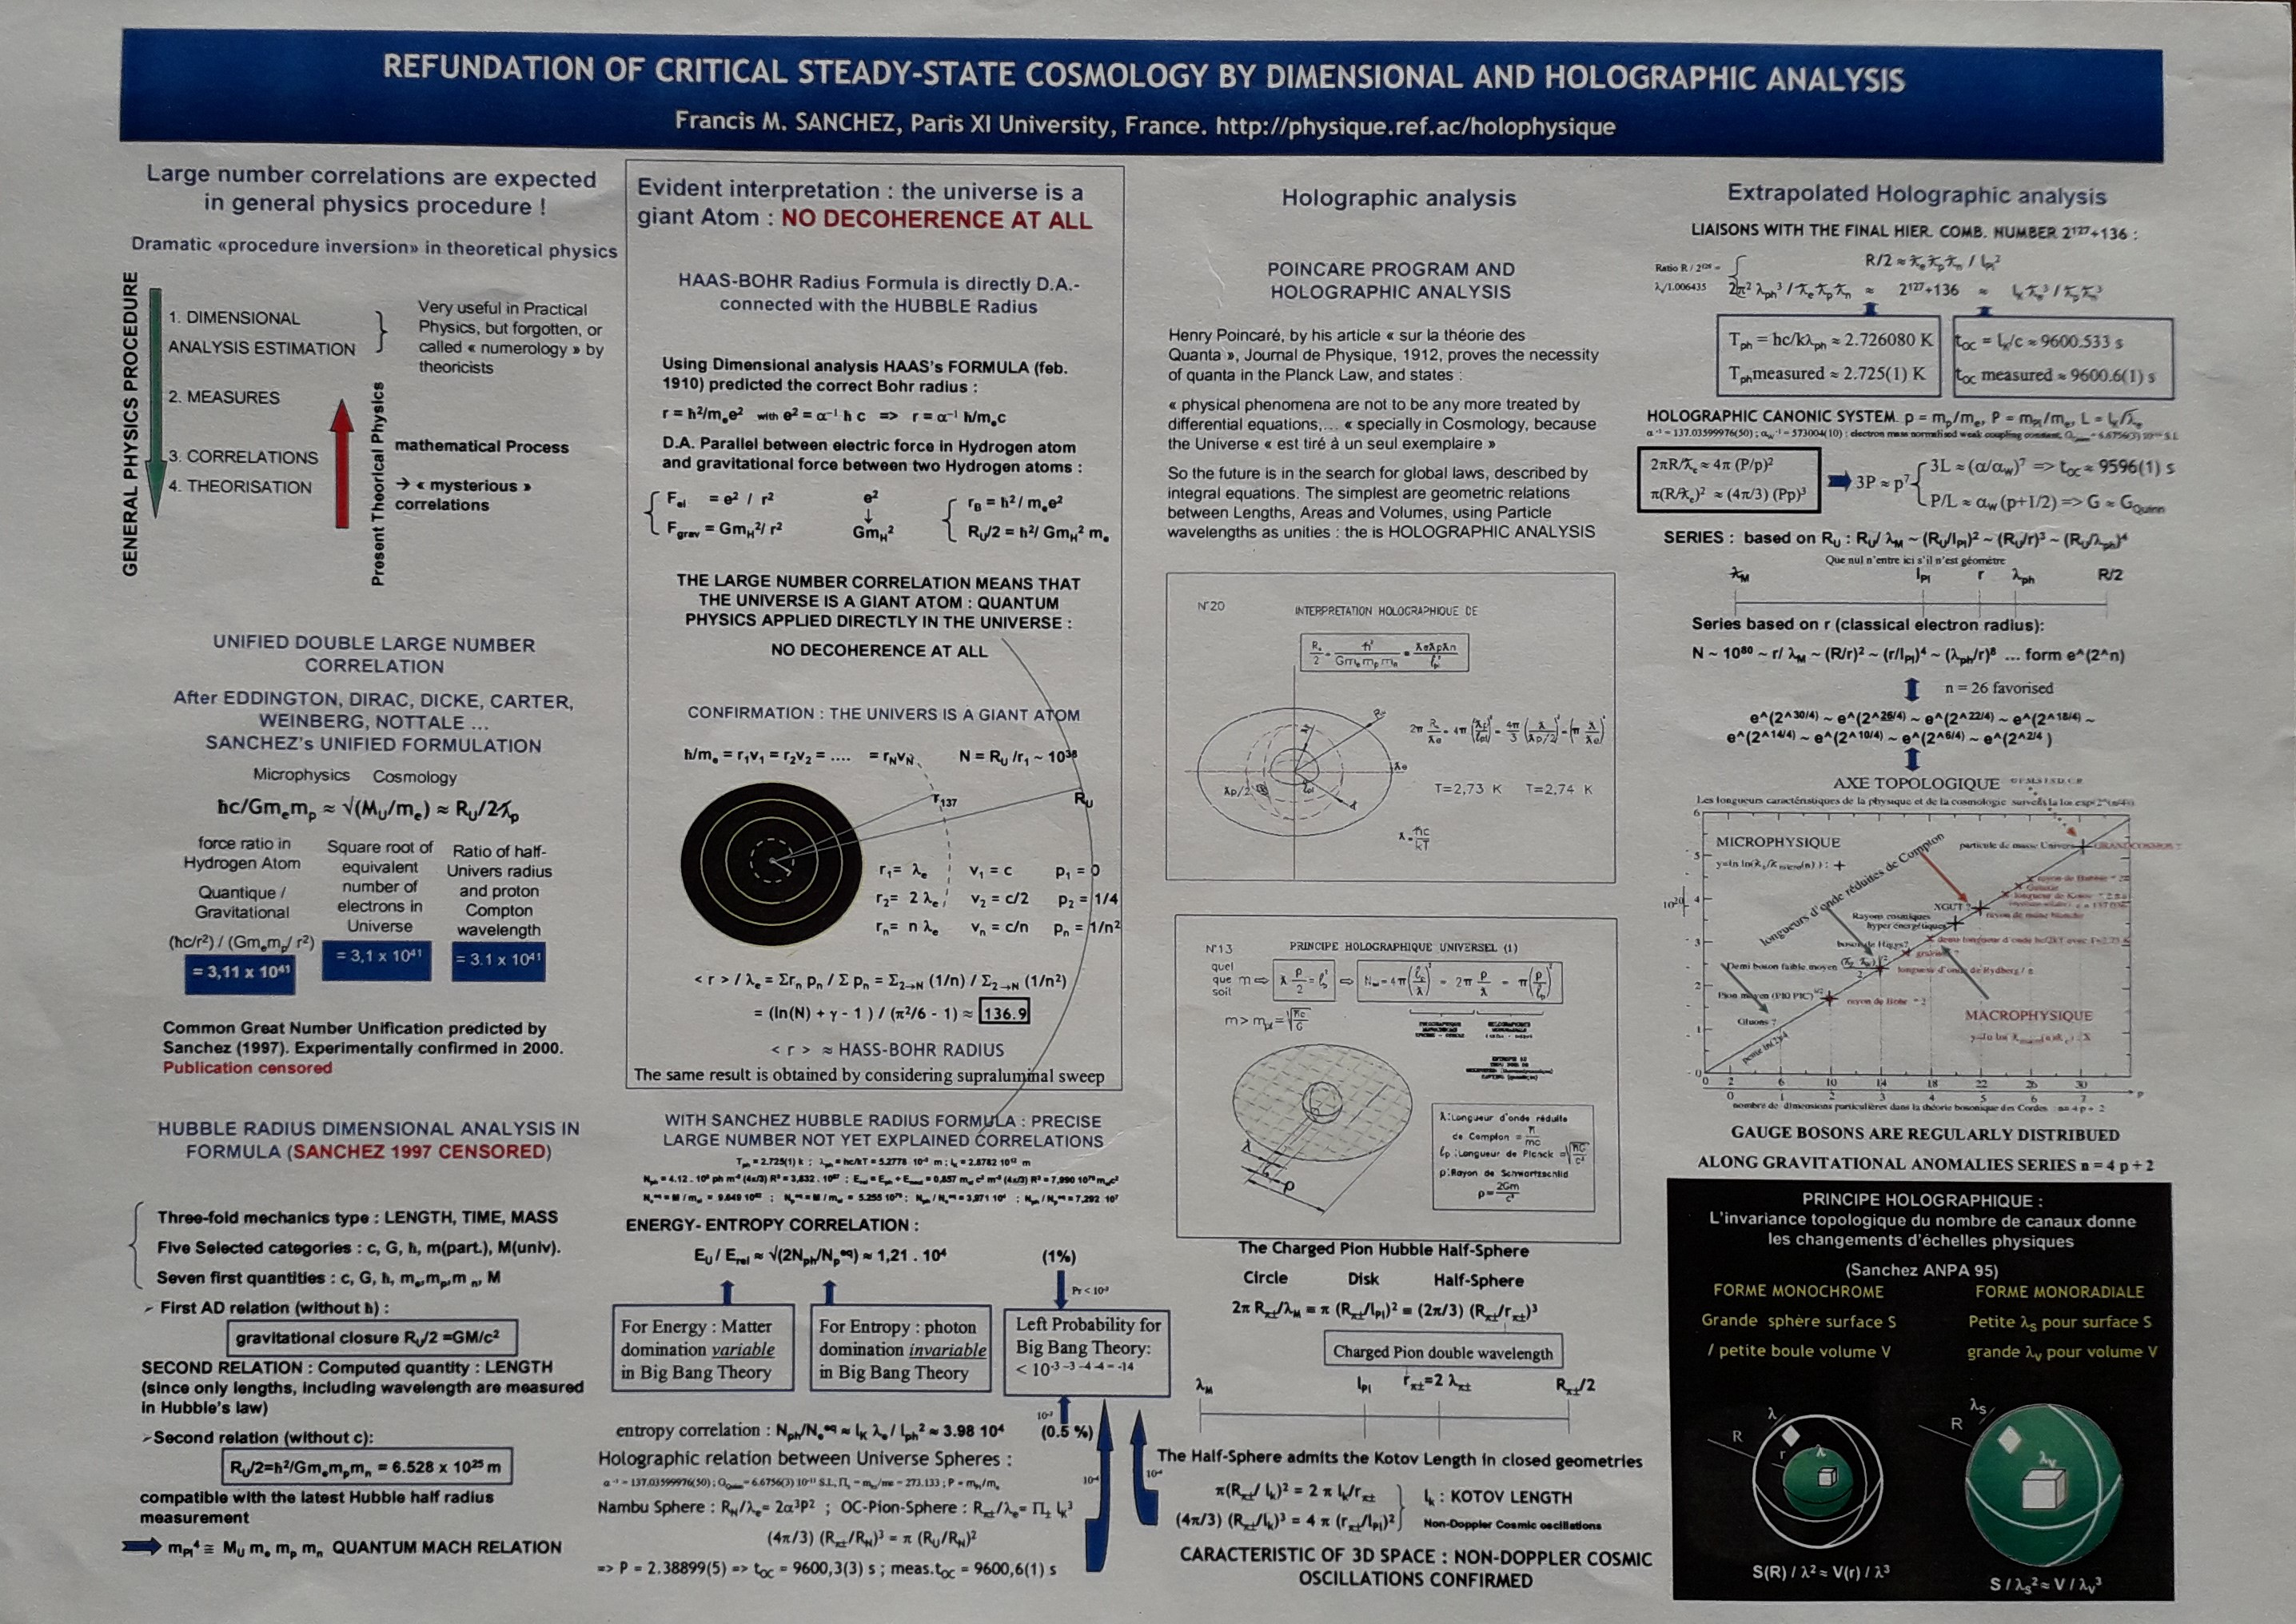
\includegraphics[width=5.5cm,height=2.5cm]{./figures/Collegedefrance2004.png}
\caption[Holophysique presentation College de France 2004]{\textit{Refundation of critical steady-state cosmology by Holographic and dimensional analysis} - Collège de France 2004.} 
\label{fig:22:figure22}
\end{figure}

%\begin{figure}
%\centering
%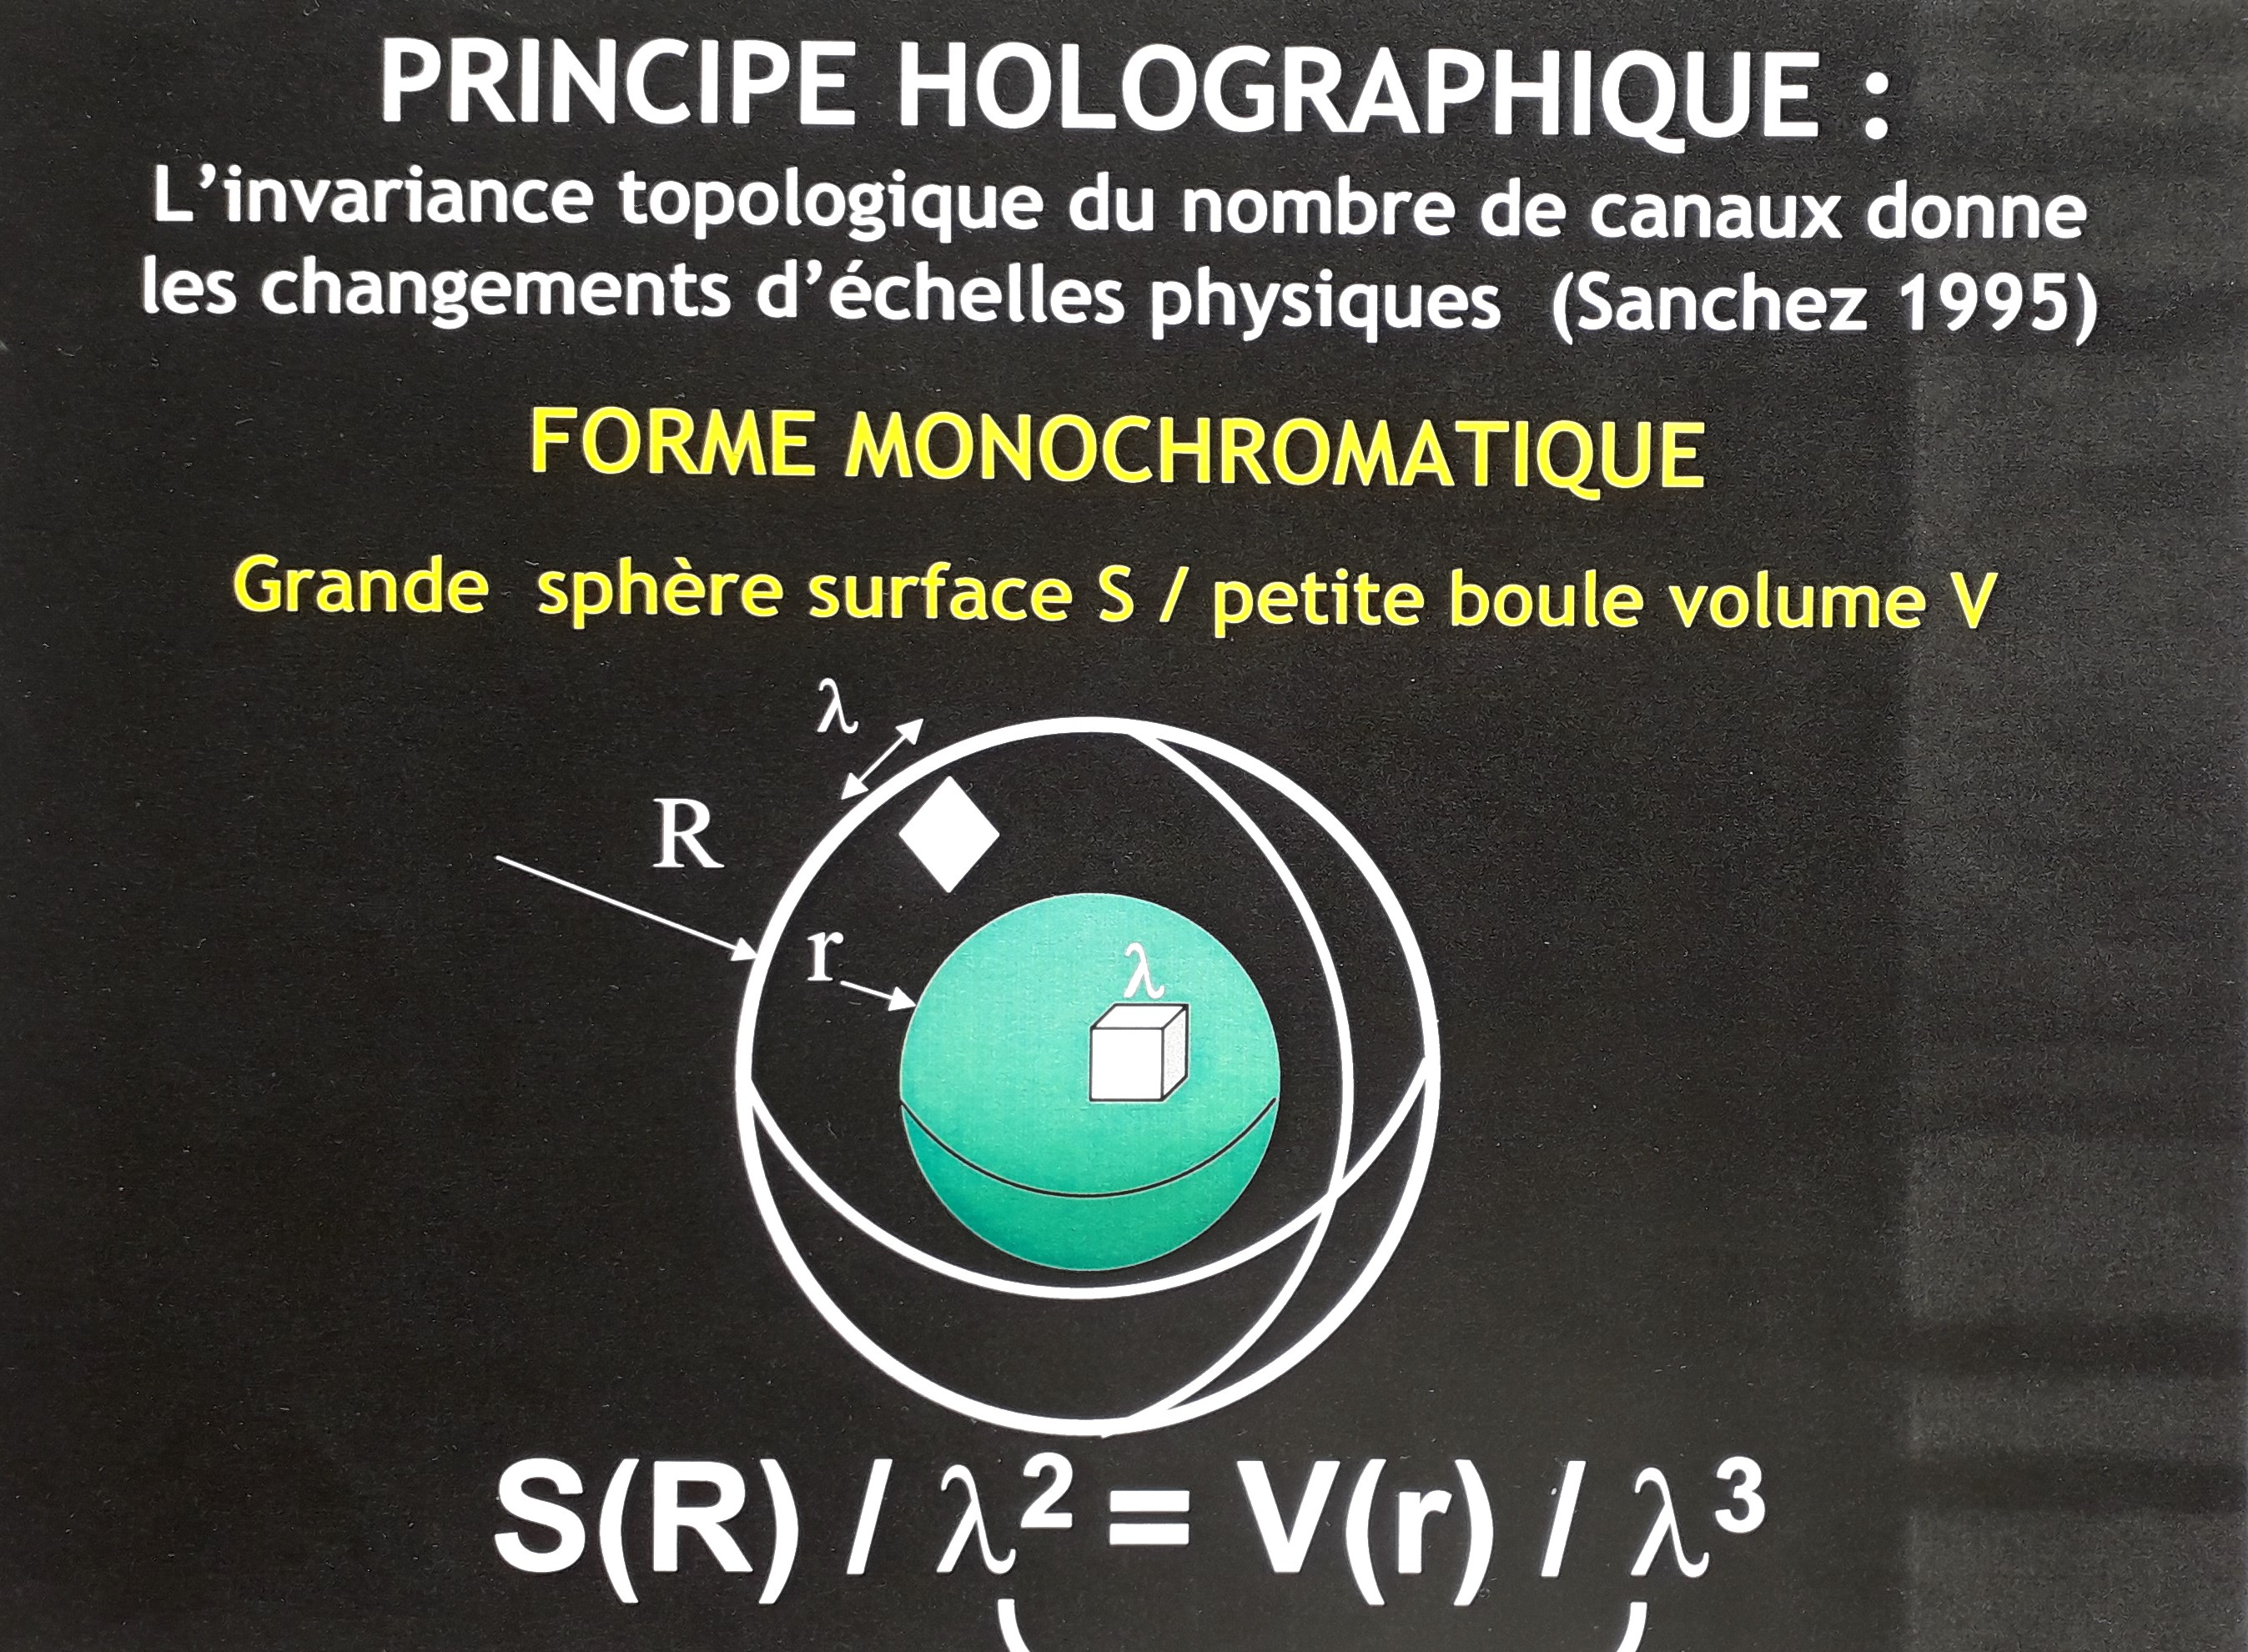
\includegraphics[width=8.5cm,height=5.5cm]{./figures/HPmonochro.jpg}
%\caption[HP monochro Collège de France 2004]{\textit{HPmonochro, College de France} - date 2004.} 
%\label{fig:23:figure23}
%\end{figure}

%\begin{figure}
%\centering
%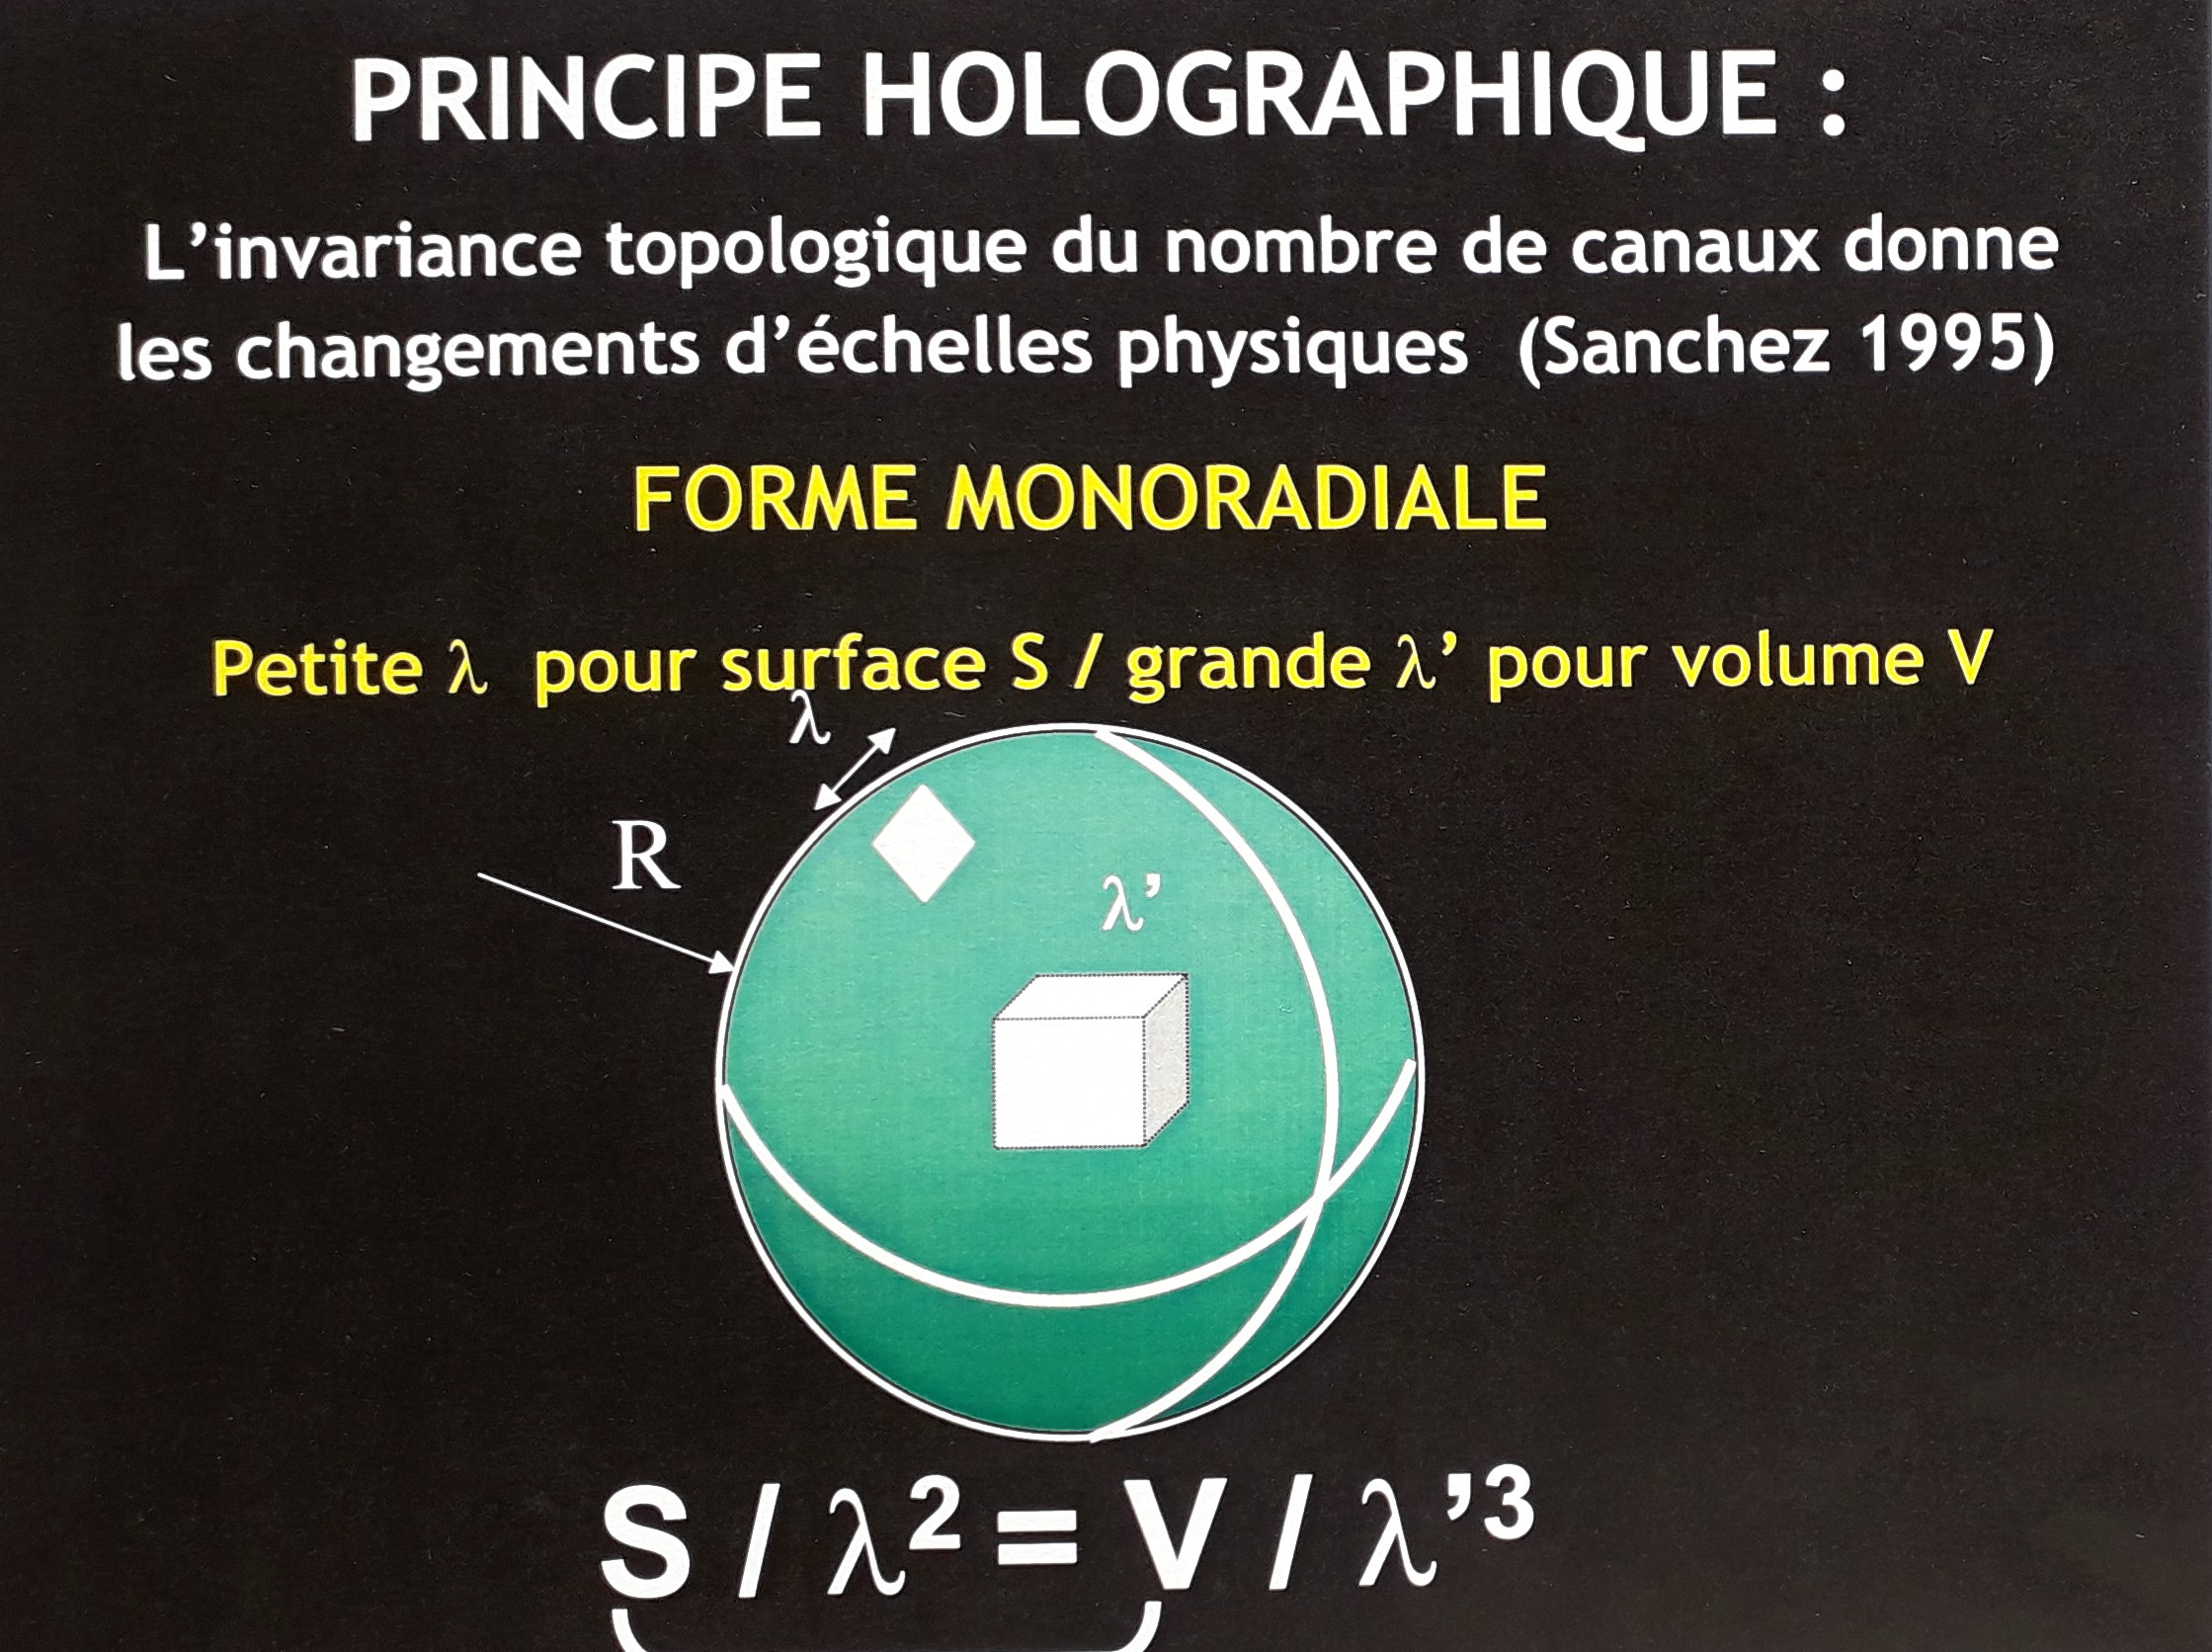
\includegraphics[width=8.5cm,height=5.5cm]{./figures/HPmonoradial.jpg}
%\caption[HP monoradial Collège de France 2004]{\textit{HPmonoradial, College de France} - date 2004.} 
%\label{fig:24:figure24}
%\end{figure}

%\begin{figure}
%\centering
%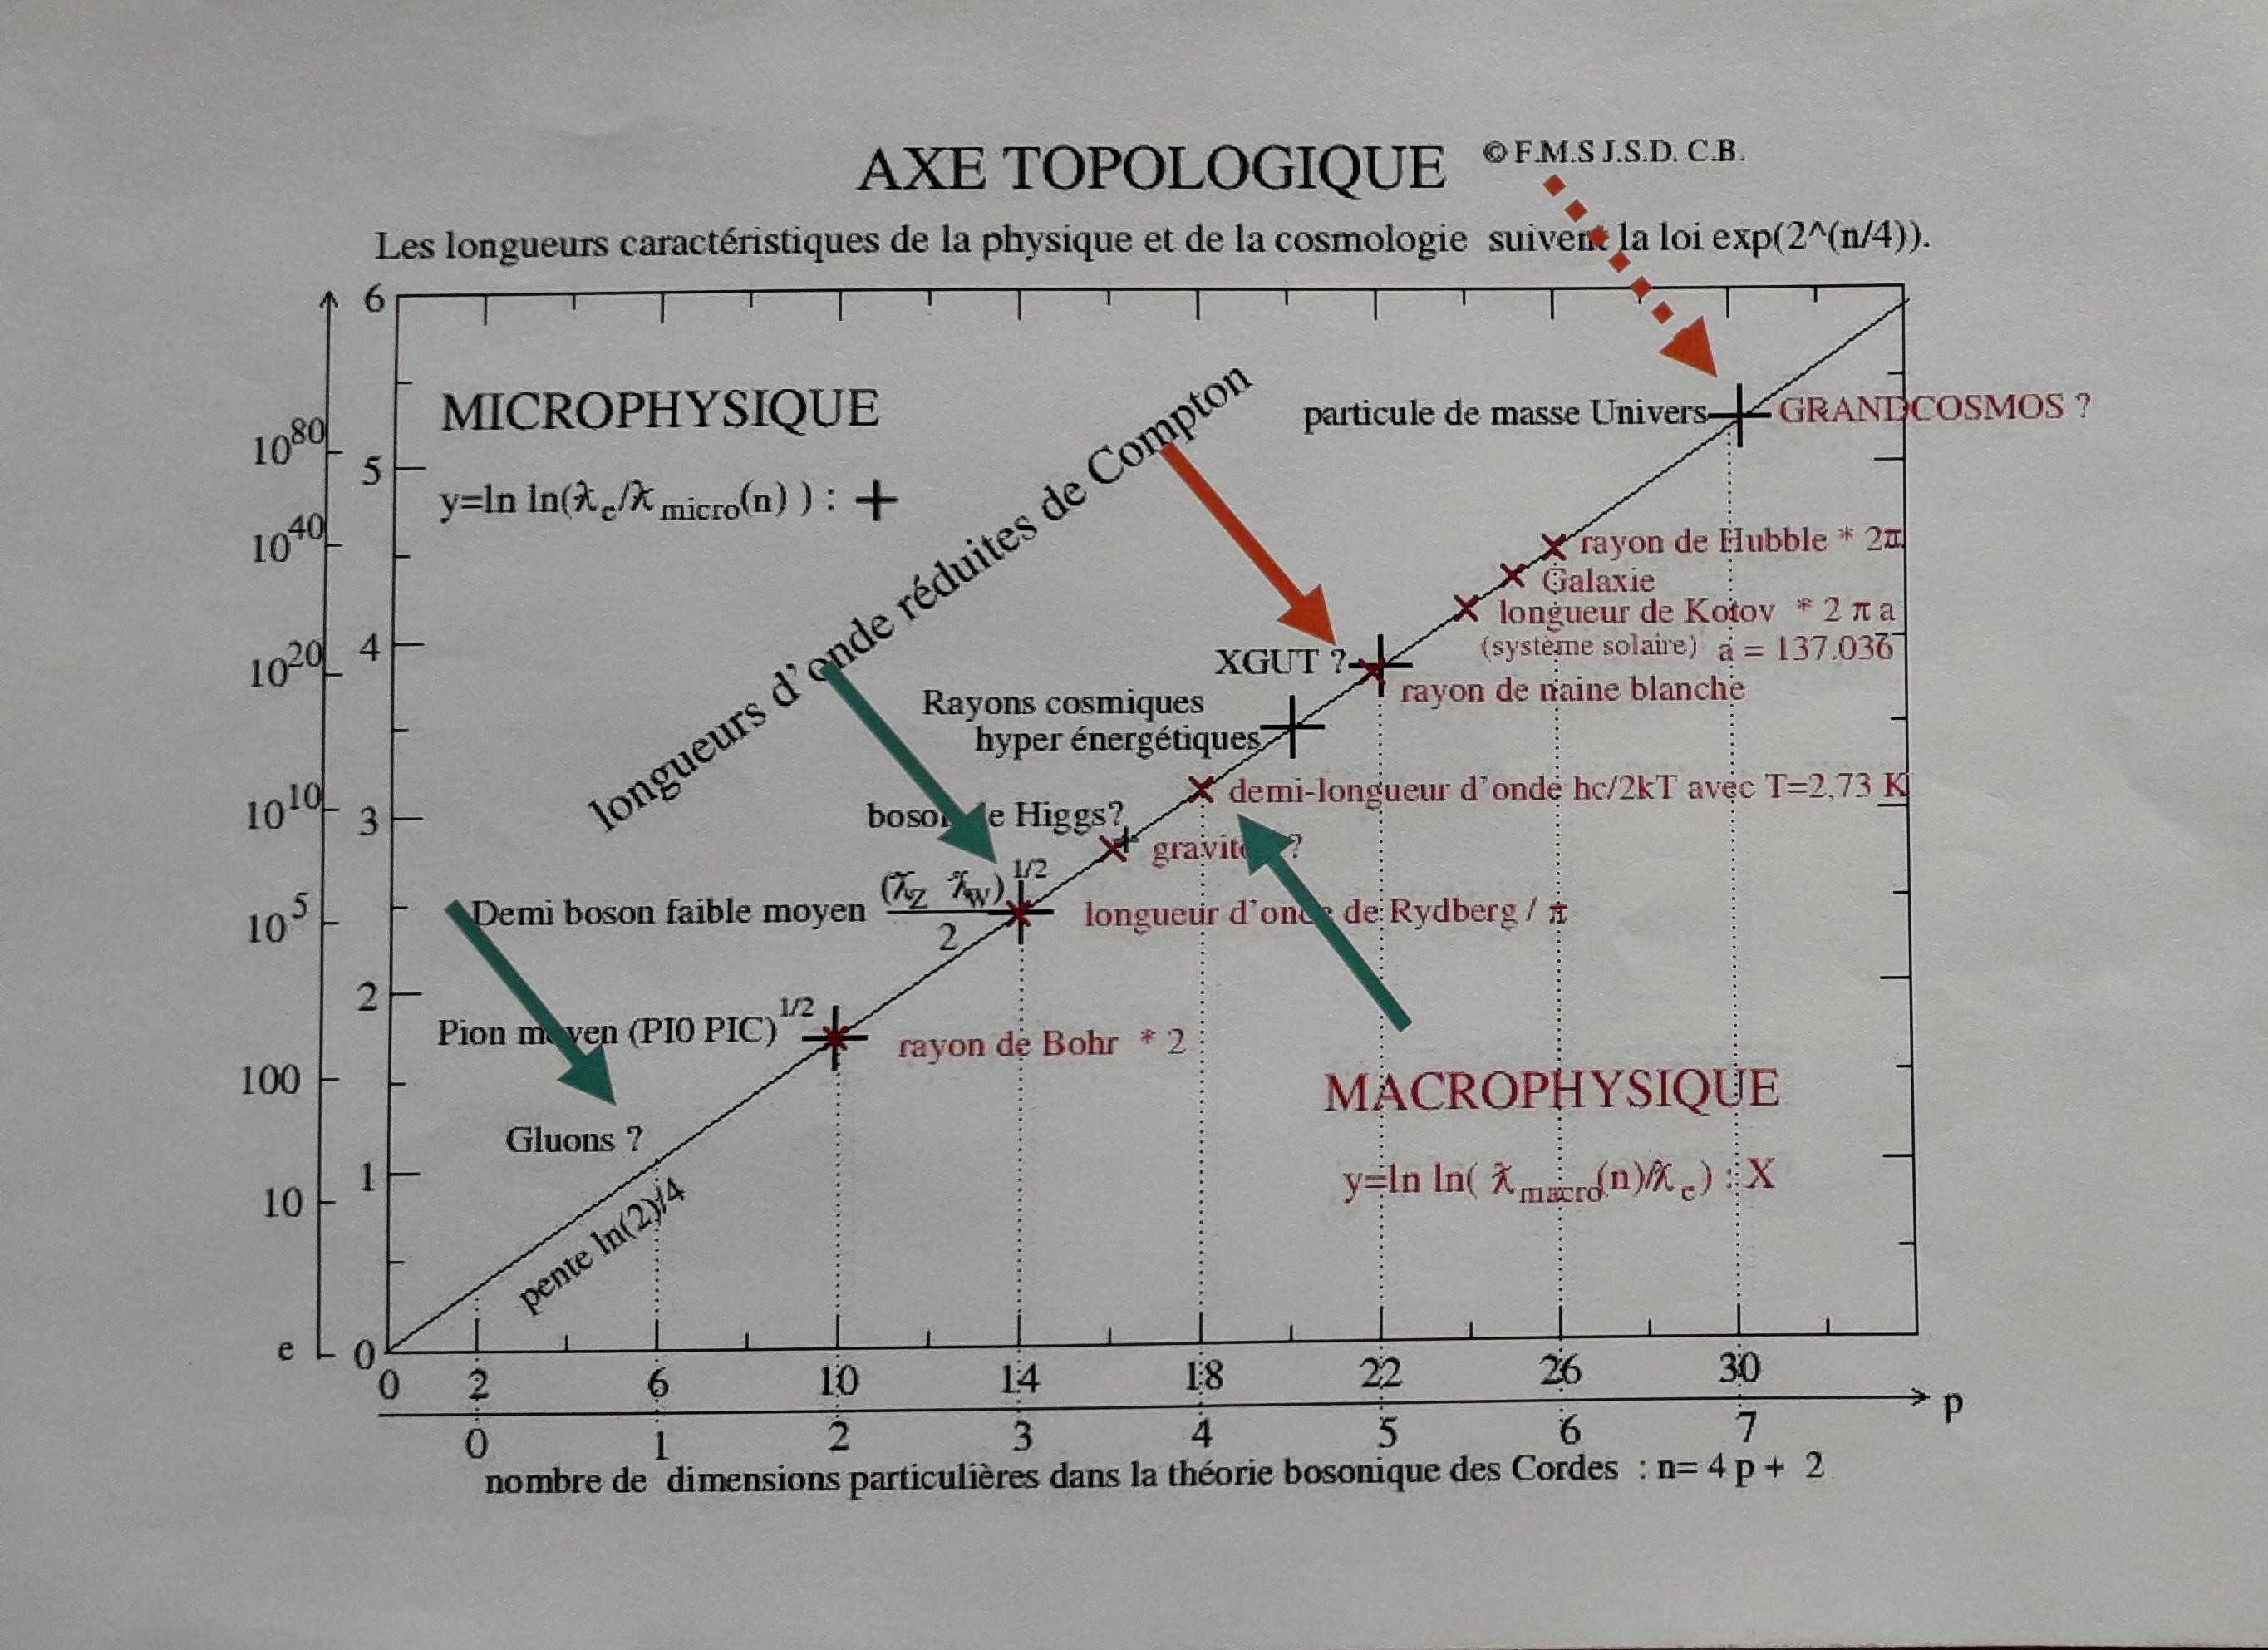
\includegraphics[width=8.5cm,height=5.5cm]{./figures/ATgaugebosons.jpg}
%\caption[Axe Topologique: Bosons de jauge, Collège de France, 2004.]{\textit{Axe Topologique: Bosons de jauge, College de France} - date 2004.} 
%\label{fig:25:figure25}
%\end{figure}

%\begin{figure}
%\centering
%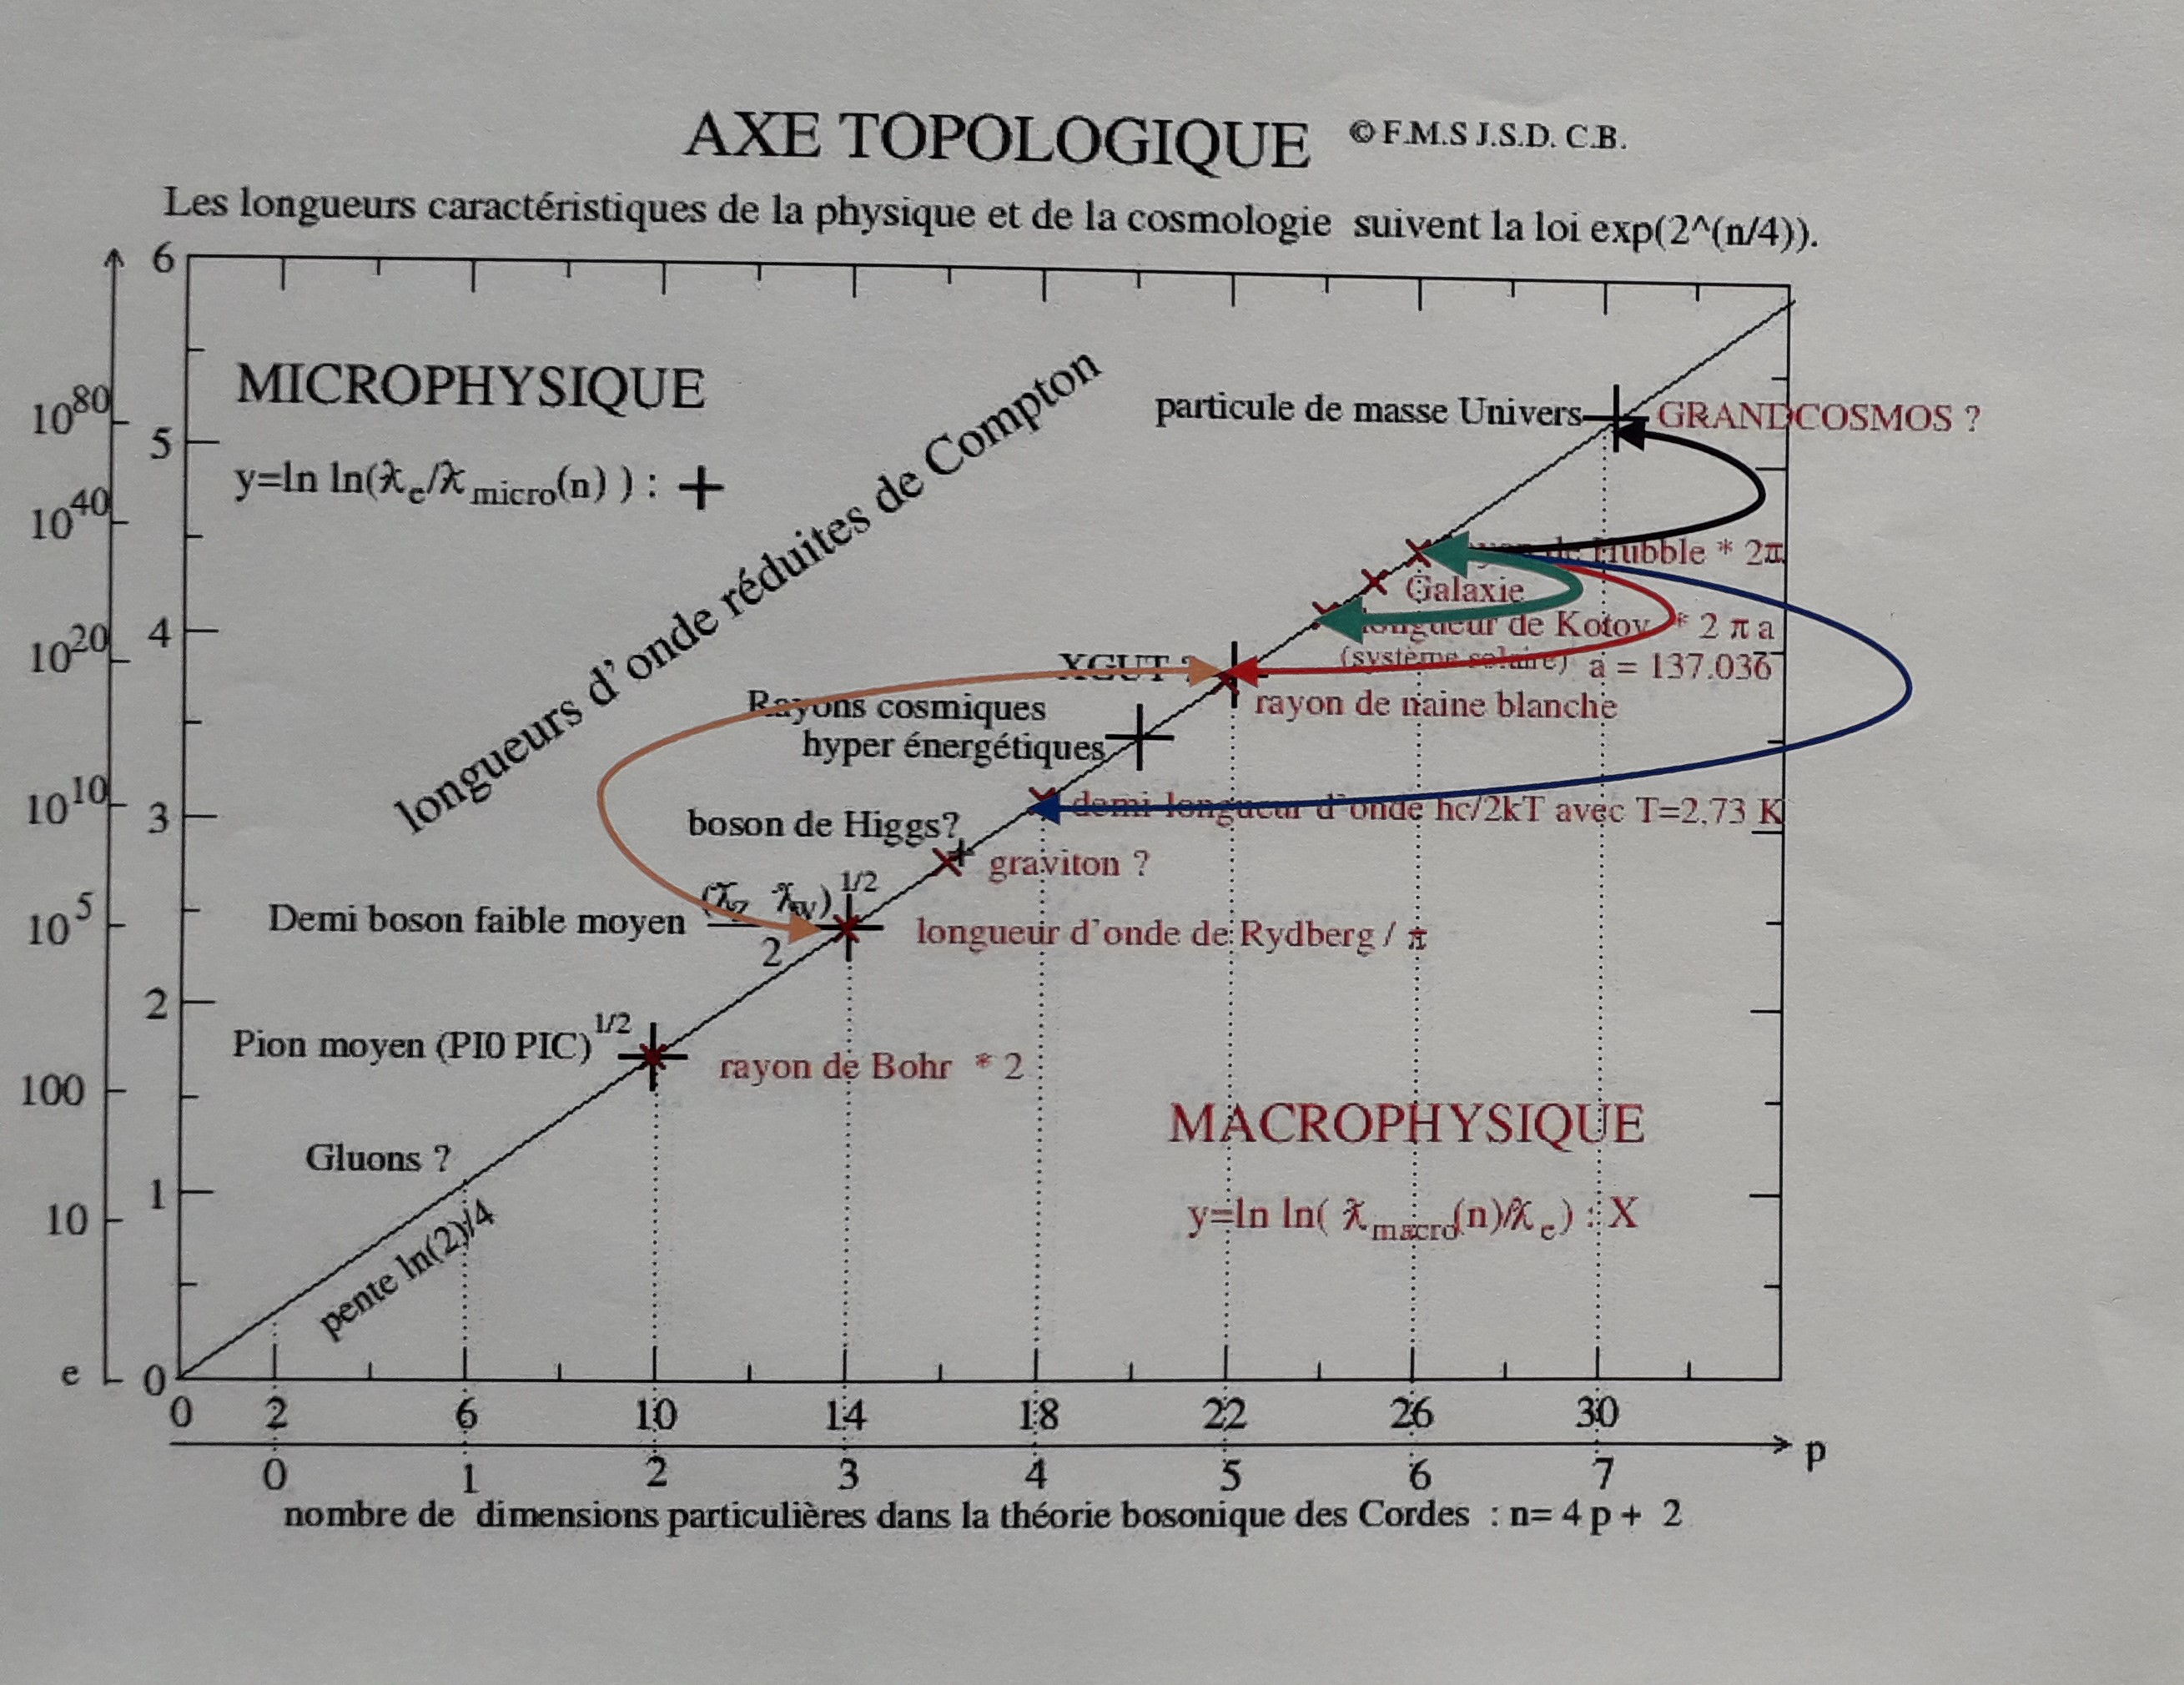
\includegraphics[width=8.5cm,height=5.5cm]{./figures/ATconexions.jpg}
%\caption[Axe Topologique: Connexions, Collège de France, 2004.]{\textit{Axe Topologique: Connexions, College de France} - date 2004.} 
%\label{fig:26:figure26}
%\end{figure}

%\begin{figure}
%\centering
%%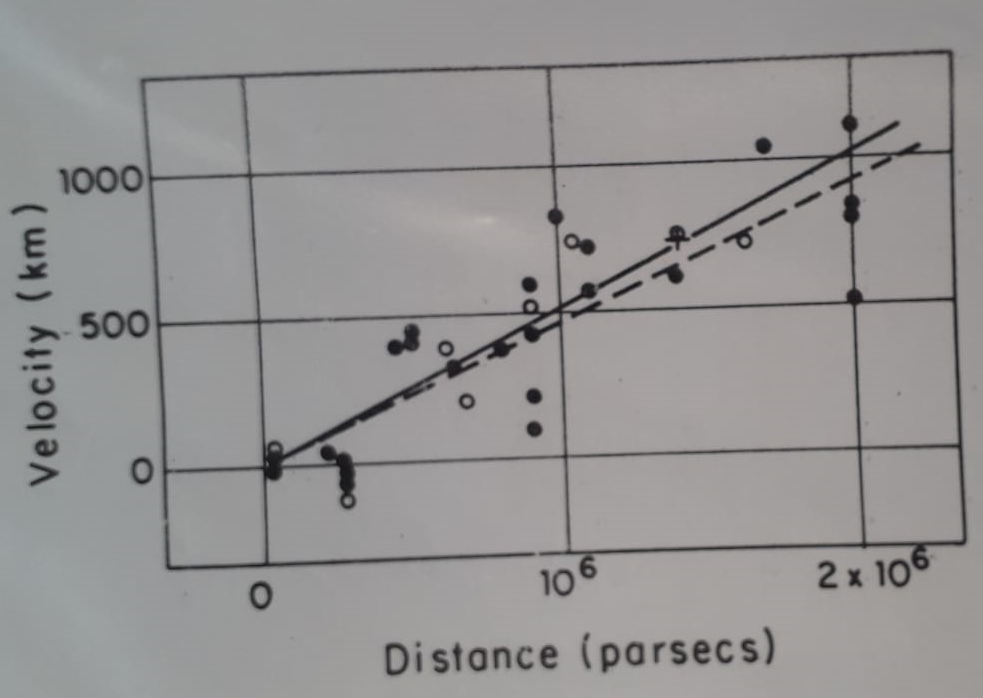
\includegraphics[width=14.5cm,height=8.6cm]{./figures/hubble-edwin-1929-ProcNaturalAcad.SciVol15p168.png}https://www.pnas.org/content/pnas/15/3/168/F2.large.jpg

%% \write18{wget https://www.pnas.org/content/pnas/15/3/168/F2.large.jpg}
%%\href{https://www.pnas.org/content/pnas/15/3/168/F2.large.jpg}{\incudegraphics{F2.large.jpg}}
%\includegraphics{hubble-orig.jpg}
%\caption [Edwin Hubble 1929]{\textit{Edwin Hubble ProcNaturalAcad-SciVol15p168} - Tracé .} 
%\label{fig:10:figure10}
%\end{figure}






\bibliographystyle{unsrt}  
%\bibliography{references}  %%% Remove comment to use the external .bib file (using bibtex).
%%% and comment out the ``thebibliography'' section.


%%% Comment out this section when you \bibliography{references} is enabled.
\begin{thebibliography}{1}

\bibitem{Sanchez3} Sanchez F.M. ``Towards the grand unified Holic Theory''. Current Issues in Cosmology. Ed. J.-C. Pecker and J. Narlikar. p. 257--260.
\newblock Cambridge Univ. Press, 2006

\bibitem{Sanchez4} Francis M. Sanchez ``Holic Principle: The coherence of the Universe`` (Sept 1995), 324--344.
\newblock Entelechies, 16th ANPA
\bibitem{Grosmann} Michel H. Grosmann and P. Meyrueis ``Optics and Photonics Applied to Communication and Processing''. SPIE.  Jan 1979.
%%\newblock Optics and Photonics Applied to Communication and Processing.
\newblock In {\em SPIE (SPIE), 1979 International Conference on}, pages . SPIE, 1979.
  
\bibitem{Grosmann2} Michel H. Grosmann, José Rebordão,  and Patrick Meyrueis, 1985,02,p761--765,Propagation Of Waves In Optical Systems: Reformulation Of Huyghens Principle For Aspheric Systems, volume 491, Proceedings of SPIE - The International Society for Optical Engineering, doi:10.1117/12.968010
\newblock In {\em Proceedings of SPIE - The International Society for Optical Engineering}. SPIE, 1985.
\bibitem{Kress} Digital Diffractive Optics: An Introduction to Planar Diffractive Optics and Related Technology, by B. Kress, P. Meyrueis, pp. 396. ISBN 0-471-98447-7. Wiley-VCH , October 2000.
\newblock An Introduction to Planar Diffractive Optics and Related Technology.
\bibitem{Sanchez5} F. M. Sanchez, V. Kotov, M. H. Grosmann, D. Weigel, R. Veysseyre, C. Bizouard, N. Flawisky, D. Gayral, L. Gueroult, ``Back to Cosmos''
\newblock {\em Progress in Physics}, 2019 (vol. 15), issue 2, http://www.ptep-online.com/2019/PP-57-12.PDF
\bibitem{Denisyuk} Yuri N. Denisyuk, ``Fundamentals of Holography'', p26--55
\newblock {\em State Optical S.I. Vavilov Institute}, 1978.
\bibitem{Tarasov} Lev V. Tarasov, ``Laser age in Optics'', p202
\newblock {\em Mir Publishers Moscow}, 1981.
\bibitem{Vienot} J-C Vienot, P. Smigielski, H. Royer ``Holographie Optique, Developpements-Applications'', preface de Dennis Gabor
\newblock {\em Dunod Ed.}, 1971.
\bibitem{Bjelkhagen} Hans I. Bjelkhagen, H. John Caulfield ``Selected Papers on Fundamental Techniques in Holography'', Holographic Cinematography: Principle of the holographic cinematography Victor G. Komar (in 1st European Congress on Optics Applied to Metrology, M. H. Grosmann, editor, 1977) p258, Vol. MS171
\newblock {\em SPIE Ed.}, 2001, https://spie.org/Publications/Book/436130
\bibitem{Gabor} Dennis gabor ``Nobel Lecture: Holography'', 1948–1971. Nobel Foundation.
\newblock {\em Nobel Media AB}, 2014.
\bibitem{French} A P French; G Delacote; J Souchon-Rouyer; Alfred Kastler; J B Yelnick; et al ``Einstein : le livre du centenaire''
\newblock {\em Hier et Demain}, 1979.
\bibitem{Koyre} A. KOYRÉ, ``Etudes d’Histoire de la pensée scientifique'', Paris, Gallimard, 1973, p. 54.
\newblock {\em Gallimard}, 1973.
\bibitem{Sherrard} Ph. SHERRARD, ``Human Image : World Image. The death and resurrection of sacred cosmology'', Limni, Evia, Grèce, Denise Harvey, 2004, (princeps par Golgonooza Press en 1992)
\newblock {\em Golgonooza Press}, 1992.
\bibitem{Galilee} GALILÉE, ``Il Saggiatore, in Le Opere di Galileo Galilei'', Ed ; Nazionale, A. Favaro, Florence, 21 vol., 1890-1909, vol. VI, p. 232.
\newblock {\em Ed Nazionale}, 1890-1909.
\bibitem{Beaty} William J. Beaty ``Drawing Holograms by Hand'' W. T. Plummer and L. R. Gardner, "A mechanically generated hologram", Applied Optics Vol.31, No. 31 (1 November 1992) pp.6585-6588
\newblock {\em http://holowiki.nss.rpi.edu/wiki/Scratch-O-Gram}, 1992.

\bibitem{ISL}  https://www.isl.eu
\newblock {\em https://www.isl.eu/documentation/rapports-annuels}, 1958.

\bibitem{Wu}  Junfei Wu et al. ``Progress in Precise Measurements of the Gravitational Constant''
\newblock {\em https://onlinelibrary.wiley.com/doi/full/10.1002/andp.201900013}, April 2019

\bibitem{Tanabashi} M. Tanabashi et al. ``The Review of Particle Physics''
\newblock {\em http://pdg.lbl.gov/2019/reviews/rpp2019-rev-history-plots.pdf}, 2019

\bibitem{Ives} Herbert IVES, Journal of the Optical Society of America Vol. 42, Issue 8, pp. 540-543 
\newblock {\em https://doi.org/10.1364/JOSA.42.000540}, 1952

\bibitem{Lecompte} F. Sanchez C. Lecompte ``Q-Switched $Nd^3+$ Glass Laser of Variable Temporal Coherence'', Applied optics, vol.13, 05.1974, p1071--1076
\newblock {\em https://doi.org/10.1364/AO.13.001071}

\bibitem{Mainfray} C. Lecompte, G. Mainfray, C. Manus, F. Sanchez ``Laser temporal-coherence effects on multiphoton ionization processes'', Physical Review A 11(3), vol.11, 03.1975
\newblock {\em https://journals.aps.org/pra/abstract/10.1103/PhysRevA.11.1009}

\bibitem{Gabrielse} G. Gabrielse et al,, ``New Determination of the Fine Structure Constant from the Electron g Value and  QED'',  Phys. Rev. Lett. 97, 030802 (2006)
\newblock {\em http://hussle.harvard.edu/~gabrielse/gabrielse/papers/2006/NewFineStructureConstant.pdf}, 2006

\bibitem{Merkatas} C. Merkatas et. al., ``Consensus Value for the Newtonian Constant of Gravitation'' Xiv:1905.09551v1 [physics.data-an] 23 May 2019
\newblock {\em https://arxiv.org/abs/1905.09551v1}, 2019

\bibitem{Grosmann3} Grosmann, Michel and Rebordão, José and Meyrueis, Patrick., ``Propagation Of Waves In Optical Systems: Reformulation Of Huyghens Principle For Aspheric'' Proceedings of SPIE - The International Society for Optical Engineering,vol.491, 02.1985, p761--765
\newblock {\em https://www.spiedigitallibrary.org/conference-proceedings-of-spie/0491/1/Propagation-Of-Waves-In-Optical-Systems--Reformulation-Of-Huyghens/10.1117/12.968010.short?SSO=1}, 1985

\bibitem{Gentet} Yves Gentet, Philippe Gentet: Ultimate emulsion and its applications: A laboratory-made silver halide emulsion of optimized quality for monochromatic pulsed and full color holography.
\newblock {\em https://www.spiedigitallibrary.org/conference-proceedings-of-spie/4149/1/Ultimate-emulsion-and-its-applications--a-laboratory-made-silver/10.1117/12.402459.short?SSO=1}, OCT 2000

\end{thebibliography}
\end{appendix}

\end{document}
